\documentclass[english,11pt]{beamer}

\DeclareMathOperator{\Cov}{Cov}
\DeclareMathOperator{\Var}{Var}
\DeclareMathOperator{\E}{\mathbb{E}}
\DeclareMathOperator{\Proba}{\mathbb{P}}

\newcommand{\Covb}[2]{\ensuremath{\Cov\!\left[#1,#2\right]}}
\newcommand{\Eb}[1]{\ensuremath{\E\!\left[#1\right]}}
\newcommand{\Pb}[1]{\ensuremath{\Proba\!\left[#1\right]}}
\newcommand{\Varb}[1]{\ensuremath{\Var\!\left[#1\right]}}

% norm
\newcommand{\norm}[1]{\| #1 \|}

\newcommand{\indep}{\rotatebox[origin=c]{90}{$\models$}}





\usepackage{mathptmx,amsmath,amssymb,graphicx,bibentry,bbm,babel,ragged2e}

\makeatletter

\newcommand{\noun}[1]{\textsc{#1}}
\newcommand{\jitem}[1]{\item \begin{justify} #1 \end{justify} \vfill{}}
\newcommand{\sframe}[2]{\frame{\frametitle{#1} #2}}

\newenvironment{centercolumns}{\begin{columns}[c]}{\end{columns}}
%\newenvironment{jitem}{\begin{justify}\begin{itemize}}{\end{itemize}\end{justify}}

\usetheme{Warsaw}
\setbeamertemplate{footline}[text line]{}
\setbeamercolor{structure}{fg=purple!50!blue, bg=purple!50!blue}

\setbeamersize{text margin left=15pt,text margin right=15pt}

\setbeamercovered{transparent}


\@ifundefined{showcaptionsetup}{}{%
 \PassOptionsToPackage{caption=false}{subfig}}
\usepackage{subfig}

\usepackage[utf8]{inputenc}
\usepackage[T1]{fontenc}



\makeatother

\begin{document}

% Mod�lisation de la morphogenèse urbaine: vers une intégration des territoires et des réseaux

\title{Modeling Urban Morphogenesis: towards an integration of territories and networks}

\author{J.~Raimbault$^{1,2,\ast}$\\
\texttt{juste.raimbault@parisgeo.cnrs.fr}
}


\institute{$^{1}$UMR CNRS 8504 G{\'e}ographie-cit{\'e}s\\
$^{2}$UMR-T IFSTTAR 9403 LVMT
}


\date{GoPro 2017\\\smallskip
ENS Lyon\\\smallskip
December 14th 2017
}

\frame{\maketitle}





%%%%%%%%%%%%%%%%%%%
%% ABSTRACT
%\textbf{Keywords : }\textit{Urban and Network Morphogenesis Modeling ; Interactions between Networks and Territories ; Co-evolution}





%%%%%%%%%%%%%%%%%
%\section{Introduction}
%%%%%%%%%%%%%%%%%



\sframe{Complex processes of Urban Morphogenesis}{

\centering

% center of Paris
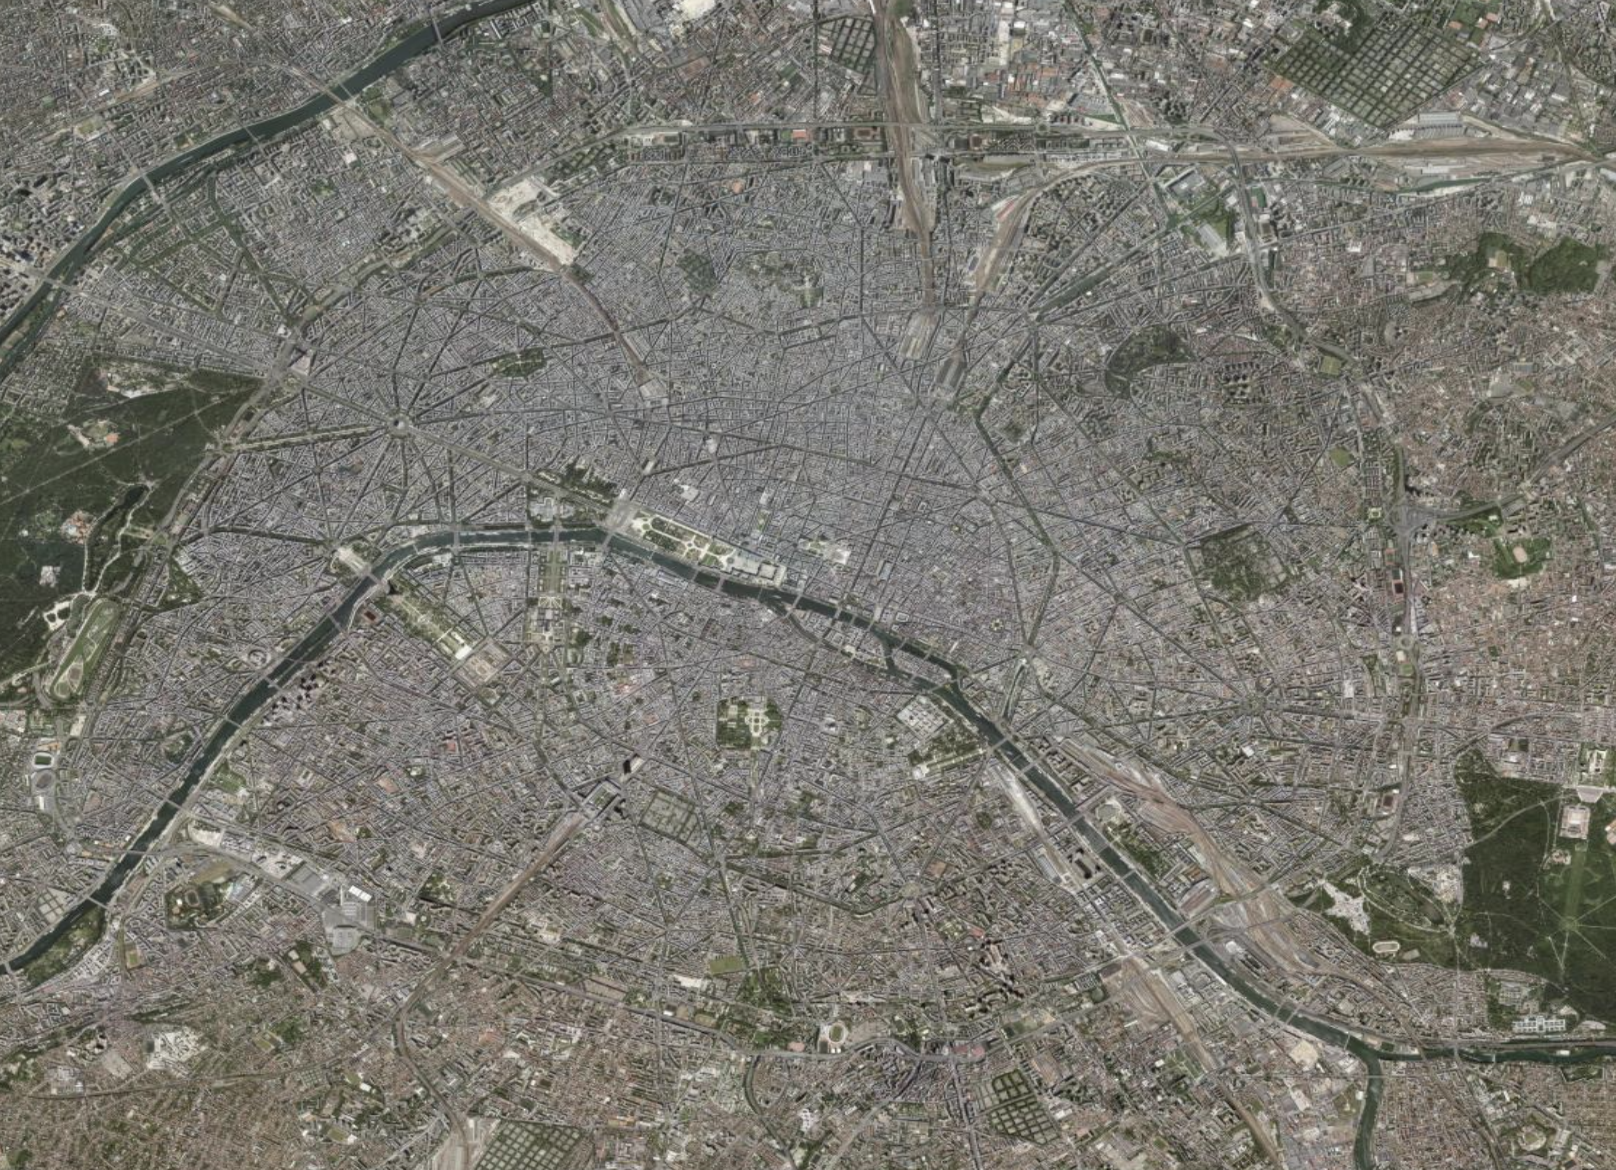
\includegraphics[width=0.9\textwidth]{figures/intro_paname}

\footnotesize\textit{Source: Geoportail}
}

\sframe{Complex processes of Urban Morphogenesis}{

\centering

% large bp
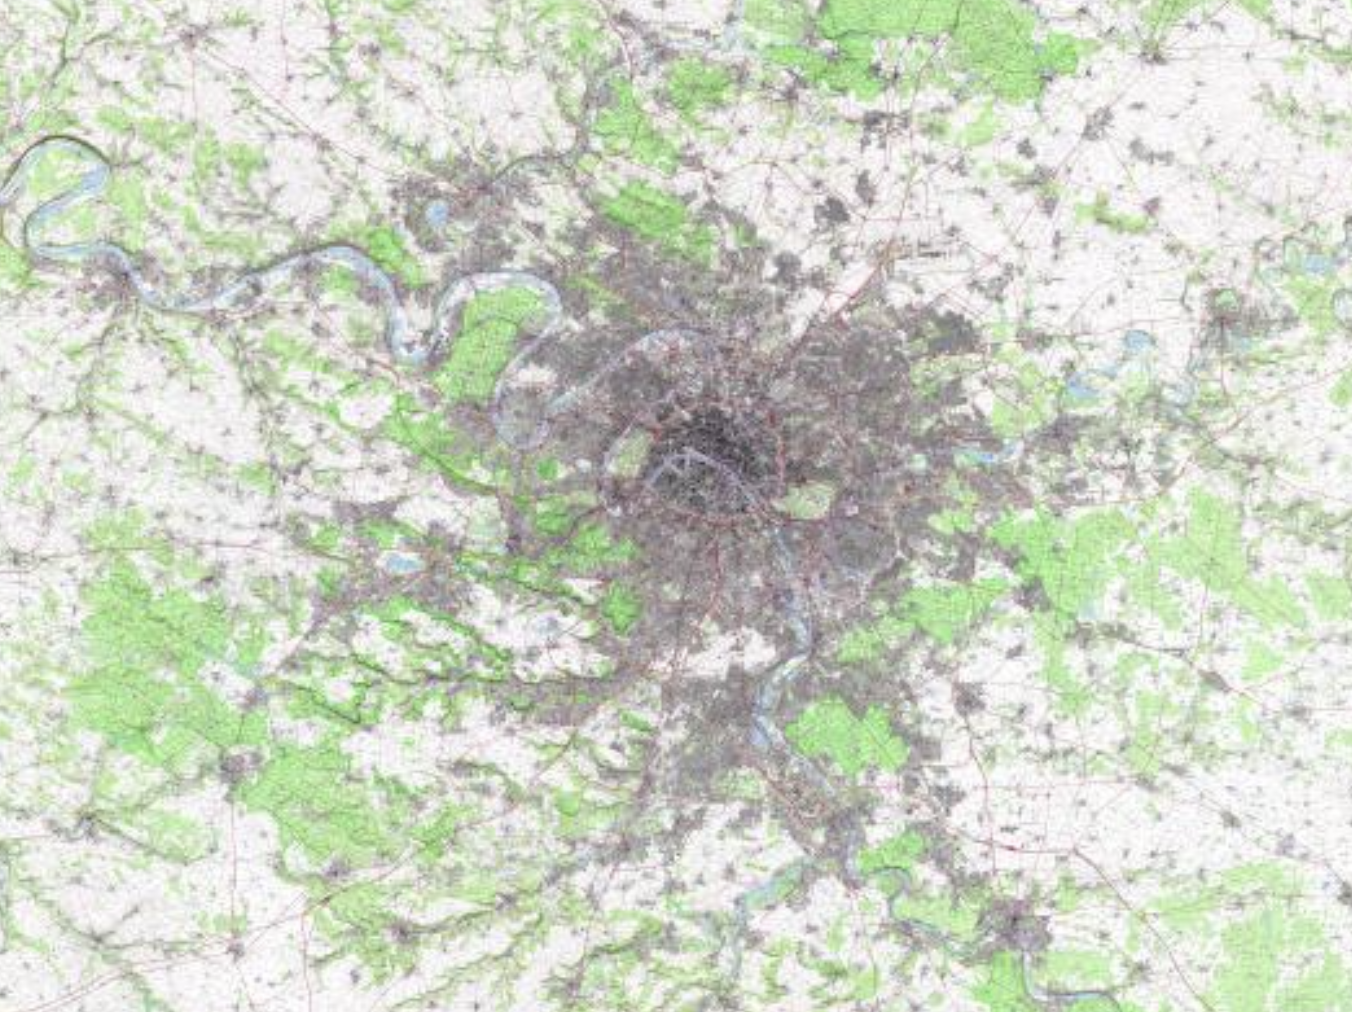
\includegraphics[width=0.9\textwidth]{figures/intro_bp}

\footnotesize\textit{Source: Geoportail}
}



\sframe{What is Morphogenesis ?}{

\textbf{Morphogenesis} (\textit{Oxford dictionary}) 
\begin{enumerate}
\item \textit{Biology} : The origin and development of morphological characteristics
\item \textit{Geology} : The formation of landforms or other structures.
\end{enumerate}

\bigskip

\textbf{History of the notion}

$\rightarrow$ Started significantly with embryology around 1930~\cite{abercrombie1977concepts} 

$\rightarrow$ Turing's 1952 paper~\cite{turing1952chemical}, linked to the development of Cybernetics

$\rightarrow$ first use in 1871, large peak in usage between 1907-1909, increase until 1990, decrease until today. \textit{Scientific fashion ?}


}



\sframe{Modeling Urban Morphogenesis}{

\justify

\cite{makse1998modeling} correlated growth; 

\smallskip

\cite{10.1371/journal.pone.0133780} multi-scale migration and percolation; 

\smallskip

\cite{bonin2012modele} qualitative differentiation of urban function; 

\smallskip

\cite{achibet2014model} procedural model at the micro-scale 

\smallskip

\cite{bonin2014modelisation} urban economics morphogenesis, only work to explicitly mention the morphogen.

}



\sframe{Cellular Automata : exemples}{

\begin{figure}
\subfloat[Microeconomic model of sprawl, \cite{DBM11}]{
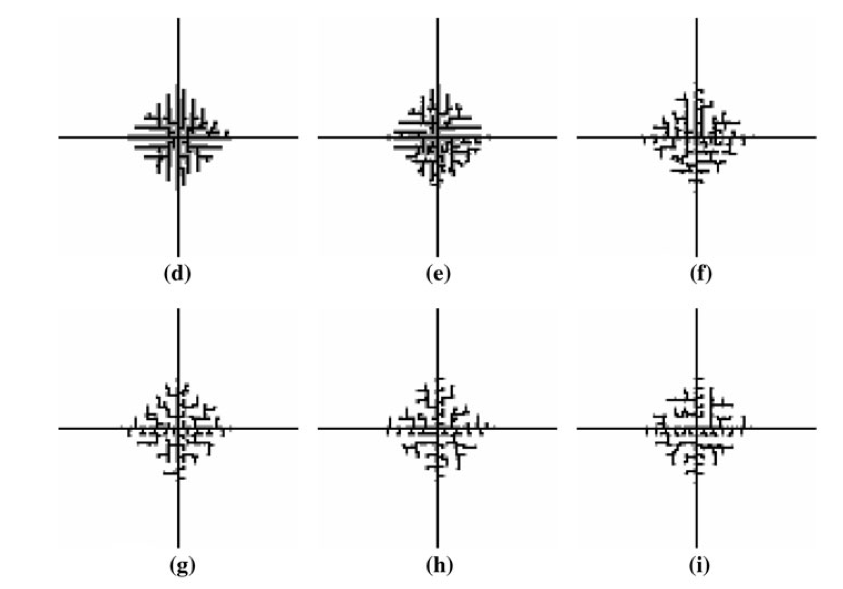
\includegraphics[trim=5cm 0cm 0cm 7cm,scale=0.23]{figures/rbd_dbmexample}}
\subfloat[Land use simulations, \cite{van2012activity}]{
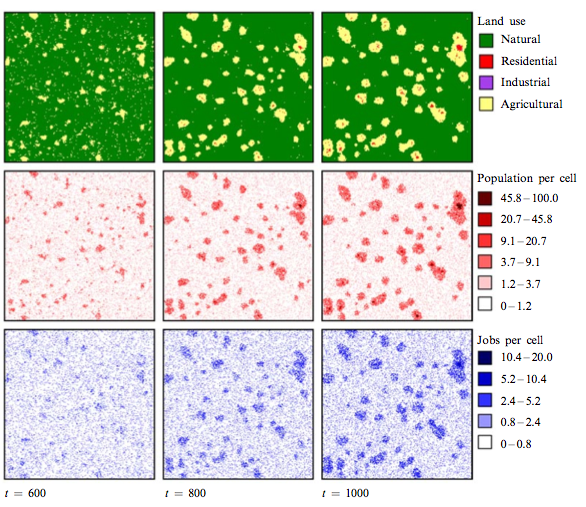
\includegraphics[trim=0cm 0cm 0cm 7cm,scale=0.27]{figures/rbd_exampleWhite}}
\end{figure}

\smallskip

\cite{DBM11} micro-economic model of sprawl

\smallskip

\cite{peeters2009space} 1D CA to show
path-dependence of settlements patterns

}


%
%\sframe{CA in Urban Planning}{
%\begin{itemize}
%\vfill{}
%
%\item \begin{justify}First introduction for reproduction of fractal urban form and land-use patterns in \cite{white1993cellular,batty1997cellular}.\end{justify}
%\vfill{}
%\item \begin{justify}Since then, numerous applications, e.g. coupling with GIS in quantitative
%geography, calibration on real land-use configurations (review in
%\cite{iltanen2012cellular}).\end{justify}
%\vfill{}
%\item \begin{justify}Examples: \cite{DBM11} micro-economic model of sprawl; \cite{peeters2009space} 1D CA to show
%path-dependence of settlements patterns;
%\cite{Wu96alinguistic} real-time rules for sustainable development.\end{justify}
%\end{itemize}
%}







\sframe{Which models for Urban Morphogenesis ?}{

% why modeling, exemple of rbd
% -> champ ; difficultés ("verrous". rq : j'aime pas la metaphore du verrou, trop cadrant et suppose que deja construit et qu'il suffit d'ouvrir. demarche epistemo de co-evol des connaissances, ni inductif ni deductif. il faut contruire. horizons d'exploration plus appropriés. rejoint l'idee de faire rentrer dans "cadre analytique" : cases prédéfinies, alors qu'il s'agit au contraire de définir ces cases. -> relire hdr arnaud

\justify

%\begin{columns}
%\column{0.4\textwidth}
%\centering
%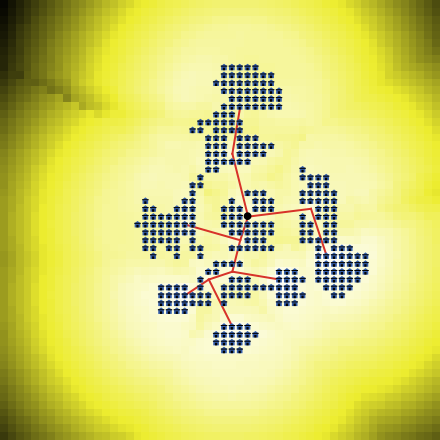
\includegraphics[width=\textwidth]{figures/intro_RBD_lattice}\\
%\footnotesize\textit{Example: a basic hybrid model based on elementary processes for density and network \cite{raimbault2014hybrid}}
%\column{0.57\textwidth}
%\justify
%\vspace{-1cm}


The relation between the form and the function is a crucial feature in Urban Morphogenesis models.

\medskip

$\rightarrow$\textit{At the crossroad between Urban Simulation and Artificial Life, few models try to integrate and explain the link between Urban Form and Function}

\medskip

$\rightarrow$\textit{Importance of parcimonious, stylized models: modeling as a tool to understand processes}


\bigskip

\textbf{Research Objective : } Explore simple models to capture morphogenesis based on abstract representation of urban processes; test their ability to reproduce existing urban systems or to optimize new systems from scratch



}


%%%%%%%%%%%%%%%%%%%%
%%%% Network Morphogenesis



\sframe{Network morphogenesis model}{

Model studied by~\cite{TeroAl10} : exploration and reinforcement by a slime mould searching for ressources

\medskip

Settings :
\begin{itemize}
	\item Initial homogeneous network of tubes $ij$ of length $L_{ij}$, variable diameter $D_{ij}$, carrying a flow $Q_{ij}$.
	\item Nodes $i$ with a pressure $p_i$.
	\item $N$ nodes are origin/destination points : randomly at each step one becomes source $p_{i_+}=I_0$ and one other sink $p_{i_-}=-I_0$
\end{itemize}


}

\sframe{Network evolution}{

At each iteration :
\begin{enumerate}
	\item Determination of flows with Kirchoff's law (electrostatic analogy) : Ohm's law $Q_{ij}=\frac{D_{ij}}{L_{ij}}\cdot(p_{i}-p_{j})$ and conservation of flows $\sum_{j\rightarrow i}Q_{ij} = 0 , \sum_{j\rightarrow i_\pm}Q_{i_{\pm}j} = \pm I_0$
	\item Evolution of diameters ($\gamma$ reinforcement parameter) by
	\[
	\frac{dD_{ij}}{dt}=\frac{\left|Q_{ij}\right|^{\gamma}}{1+\left|Q_{ij}\right|^{\gamma}}-D_{ij}
	\]
\end{enumerate}


}
  
\sframe{Network evolution}{

$\rightarrow$ Extraction of the final network after convergence given a threshold parameter for diameters (bimodal final distributions)
\medskip
$\rightarrow$ Multi-scale model : diameters are constant during an iteration to obtain equilibrium flows
%\textit{Implémentation en NetLogo ouverte~\cite{impl}}
}




\sframe{Indicators}{

Behavior of the model evaluated with performance indicators for generated network $(V_f,E_f)$, that are contradictory objectives :
          \bigskip
          \begin{itemize}
          \item Construction costs $c=\sum_{ij\in E_f}D_{ij}(t_f)$
          \bigskip
          \item \begin{justify}Average performance~\cite{banos2012towards}
          \[
          v=\frac{1}{|V_f|^2}\sum_{i,j\in V_f}\frac{d_{i\rightarrow j}}{||\vec{i}-\vec{j}||}
          \]
          \end{justify}
          \bigskip
          \item Robustness (\textit{Network Trip Robustness} index~\cite{sullivan2010identifying})
          \end{itemize}

}






\sframe{Sensitivity analysis}{

\begin{columns}[t]
        \begin{column}{.47\textwidth}
                    
          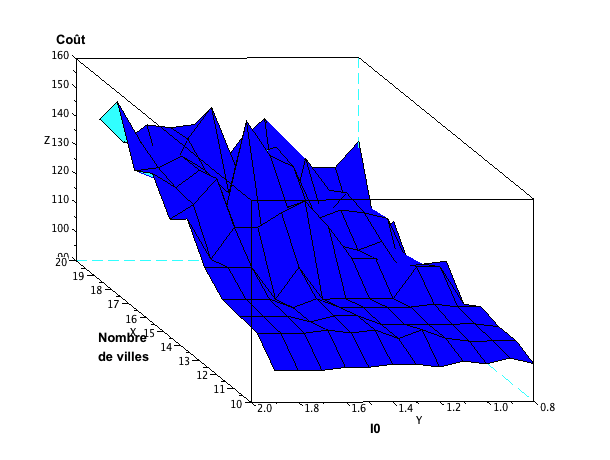
\includegraphics[width=0.5\columnwidth]{figures/slimemould_graphe_cout}
          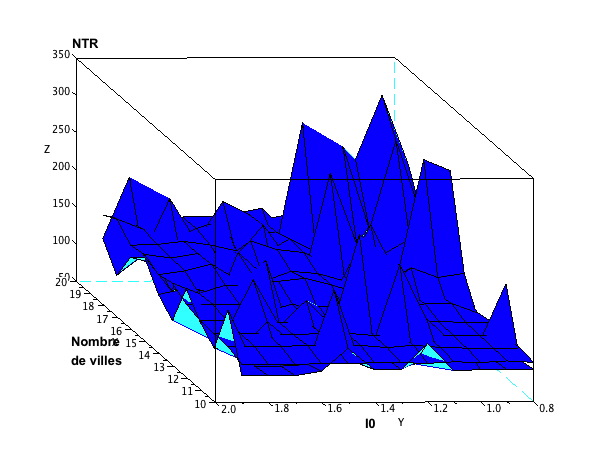
\includegraphics[width=0.5\columnwidth]{figures/slimemould_graphe_NTR}\\
          \bigskip
          \textit{Sensitivity of indicators to parameters $(N,I_0)$.}
          

          \end{column}
          \begin{column}{.47\textwidth}
          
           
            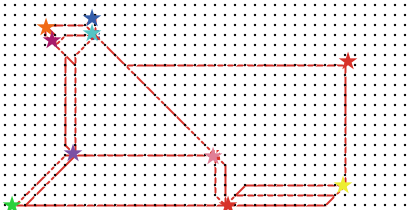
\includegraphics[width=0.5\columnwidth]{figures/slimemould_networkDense}
          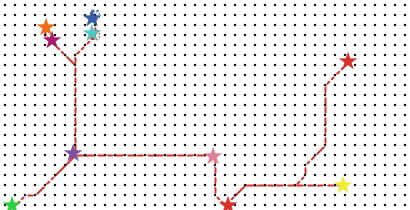
\includegraphics[width=0.5\columnwidth]{figures/slimemould_networkLessDense}\\
          \bigskip
          \begin{justify}
          \textit{Sensitivity of network topology to reinforcement coefficient $\gamma$. Left : $\gamma \sim 1$, robust network. Right : $\gamma >> 1$, arborescent network.}
          \end{justify}
          \end{column}
          \end{columns}
      
}





\sframe{Application : Corridor Optimal}{
          
Abstract application : \textit{Given a distribution of nodes to serve (sinks), what is the optimal corridor for an infrastructure at a larger scale (train or metro) for which stations are sources, in the sense of the multi-objective optimality of the local self-organized network ?}

\medskip
          
$\rightarrow$ Heuristic exploration of an arborescent set of potential infrastructures

\begin{columns}[t]
    \begin{column}{.48\textwidth}

	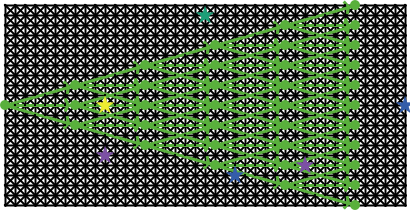
\includegraphics[width=0.5\textwidth,height=7cm]{figures/slimemould_implantationtree}
\textit{Heuristic tree to explore infrastructures.}
	\end{column}
    \begin{column}{.48\textwidth}
          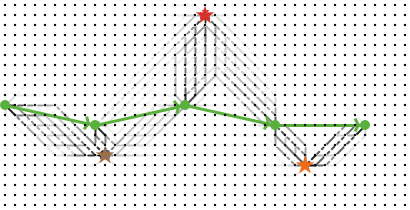
\includegraphics[width=\columnwidth,height=7cm]{figures/slimemould_ImplantationTreeview}
          
          \textit{Example of network generation for a given infrastructure.}
    \end{column}
          
\end{columns}
          
          
}
          
          
          
\sframe{Pareto Optimisation}{
          
\centering
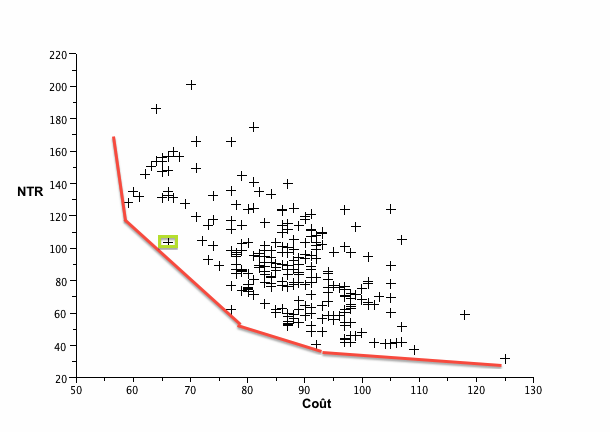
\includegraphics[width=0.33\columnwidth]{figures/slimemould_implantationcntr}
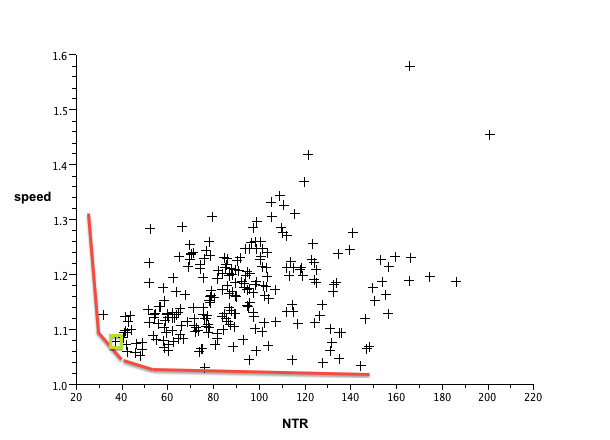
\includegraphics[width=0.33\columnwidth]{figures/slimemould_implantationntrspeed}
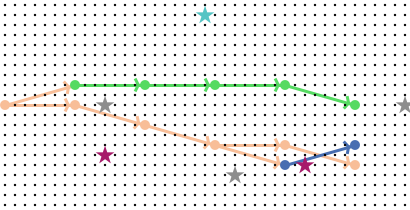
\includegraphics[width=0.33\columnwidth]{figures/slimemould_paretosimplantation}
          
\textit{Pareto optimisation : projection of explored configurations in indicator space to obtain the Pareto front ; configuration corresponding to three optimal points.}
          
}



\sframe{Application : Optimal Network Design}{

$\rightarrow$ Mission of prospective for Romainville city : itinary of an intra-urban shuttle with imposed stops.

\medskip

$\rightarrow$ NP-hard problem similar to a Travelling Salesman Problem, but multi-objective (cost, speed, robustness). The bottom-up network generation applied on the initial street network gives a compromise solution.

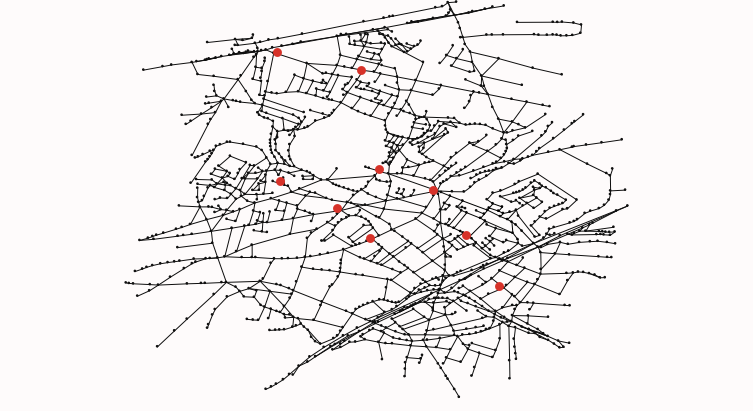
\includegraphics[width=0.32\columnwidth]{figures/slimemould_tick1}
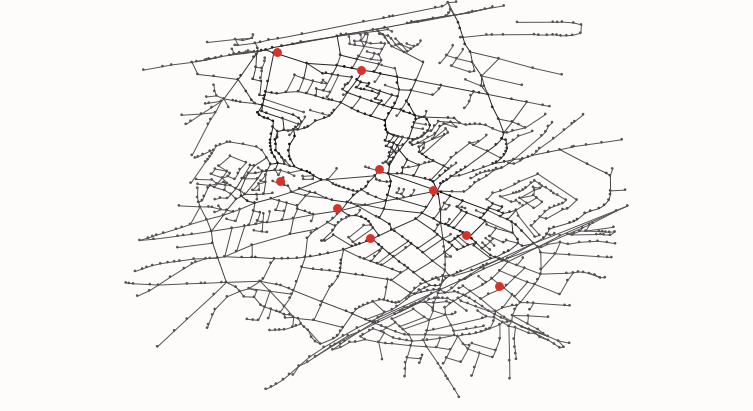
\includegraphics[width=0.32\columnwidth]{figures/slimemould_tick10}
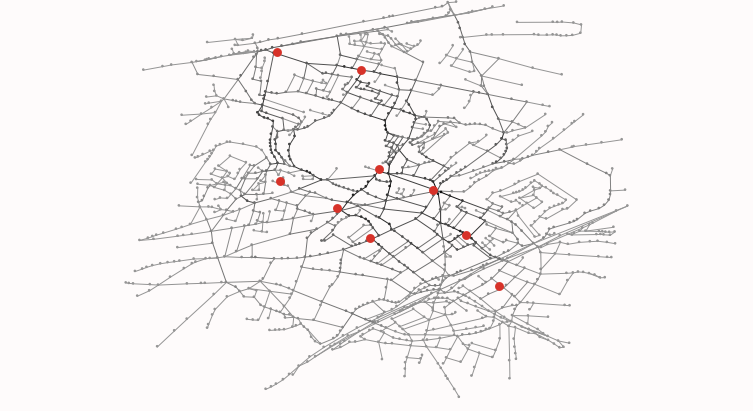
\includegraphics[width=0.32\columnwidth]{figures/slimemould_tick20}\\
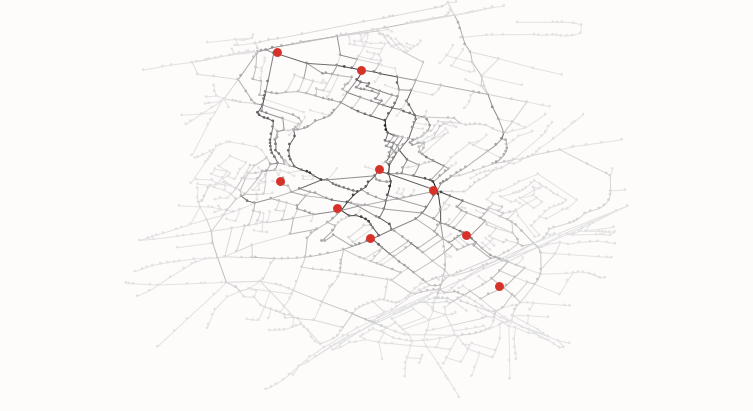
\includegraphics[width=0.32\columnwidth]{figures/slimemould_tick50}
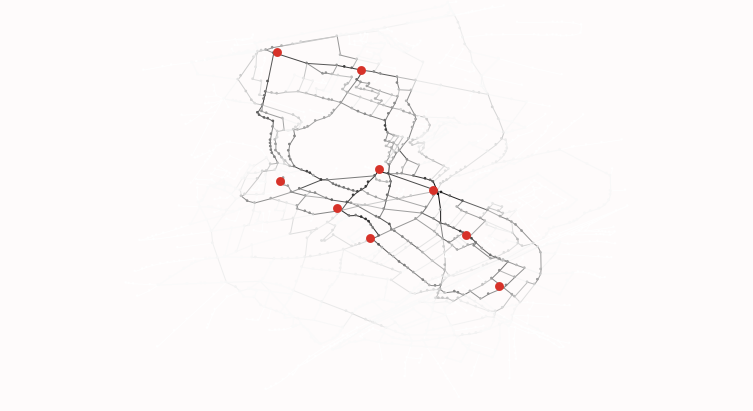
\includegraphics[width=0.32\columnwidth]{figures/slimemould_tick101}
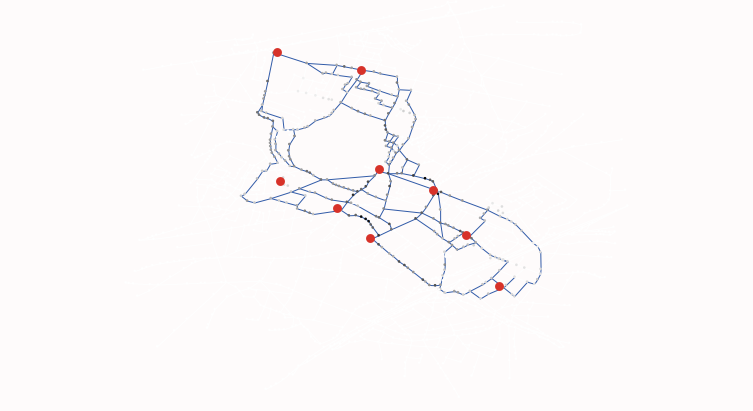
\includegraphics[width=0.32\columnwidth]{figures/slimemould_reseauFinal}\\

\textit{Progressive convergence of the network towards an optimal network connecting the fixed points (in red), starting from the initial street network.}

}





\sframe{A simple Reaction-diffusion model}{

% comment Arnaud : reaction-diffusion ?

% model rationale and processes


\justify

$\rightarrow$ Crucial role of the interplay between concentration forces and dispersion forces~\cite{fujita1996economics} in keeping Urban Systems at the border of chaos

\bigskip

$\rightarrow$ Potentiality of aggregation mechanisms (such as Simon model) to produce power laws \cite{2016arXiv160806313S}

\bigskip

$\rightarrow$ Link with Reaction-diffusion approaches in Morphogenesis~\cite{turing1952chemical}

\bigskip

$\rightarrow$ Extension of a DLA-type model introduced by \cite{batty1991generating}, with simple abstract processes of population aggregation and diffusion

}

\sframe{Model Formalization}{

% model formalization and indicators

$\rightarrow$ Grid world with cell populations $(P_i(t))_{1\leq i\leq N^2}$.

\bigskip

$\rightarrow$ At each time step:

% comment Arnaud : si tu beamais pas tu pourrais introduire une video du modèle ;-)

\begin{enumerate}
\item Population growth with exogenous rate $N_G$, attributed independently to a cell following a preferential attachment of strength $\alpha$
%\begin{equation}
%\Pb{P_i(t+1)=P_i(t)+1|P(t+1)=P(t)+1}=\frac{(P_i(t)/P(t))^{\alpha}}{\sum(P_i(t)/P(t))^{\alpha}}
%\end{equation}
%The attribution being uniformly drawn if all population are equal to 0.
\item Population is diffused $n_d$ times with strength $\beta$
\end{enumerate}

\bigskip

$\rightarrow$ Stopping criterion: fixed maximal population $P_m$.

%To avoid bord effects such as reflecting diffusion waves, border cells diffuse their due proportion outside of the world, implying that the total population at time $t$ is strictly smaller than $N_G\cdot t$.

\bigskip

$\rightarrow$ Output measured by morphological indicators: Moran index, average distance, rank-size hierarchy, entropy.


}


\sframe{Generating Population Distributions}{


% examples : fig 2 of paper

\centering

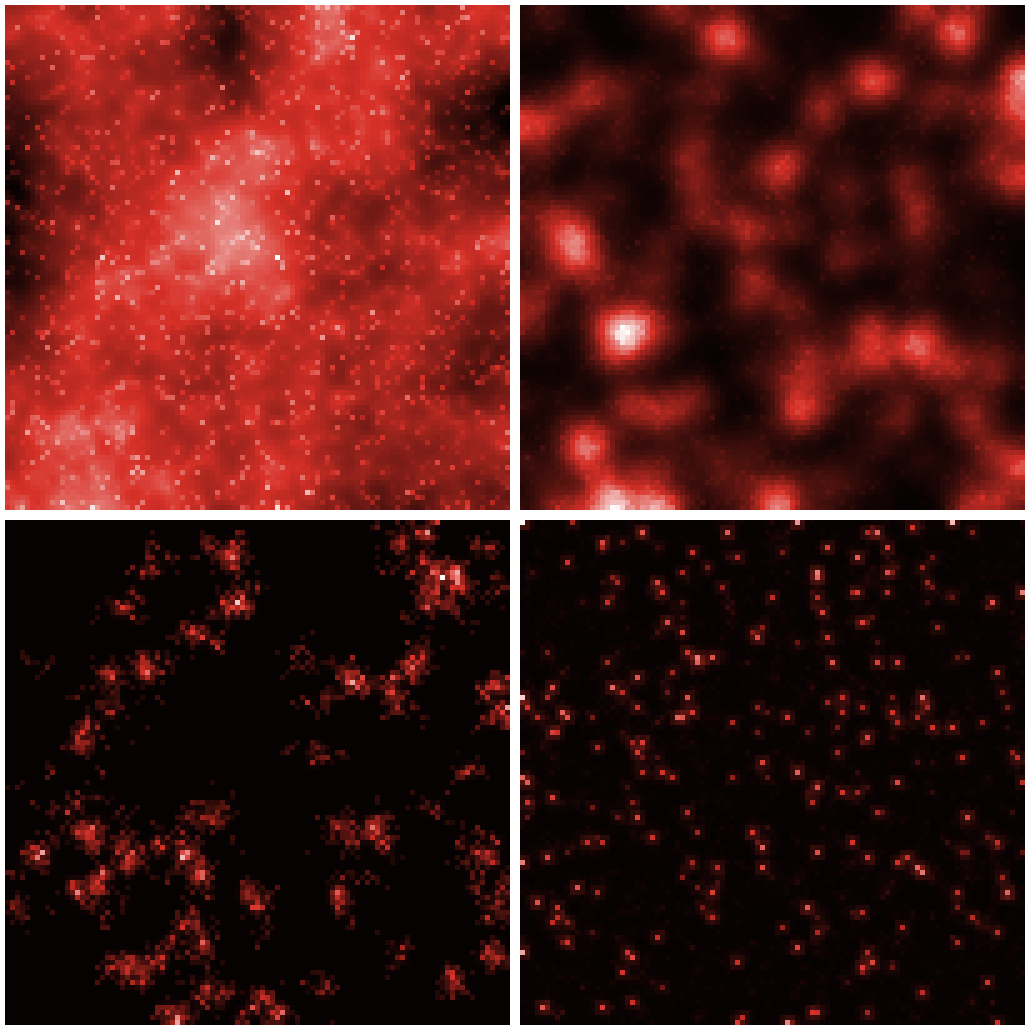
\includegraphics[height=0.8\textheight]{figures/density_Fig2}

\footnotesize\textit{Examples of generated territorial shapes}

}


\sframe{Model behavior}{

% comment Arnaud : Les graphiques correspondent aux 4 exemples précédents ? Si oui les rappeler en petite vignette. -> NON

\centering

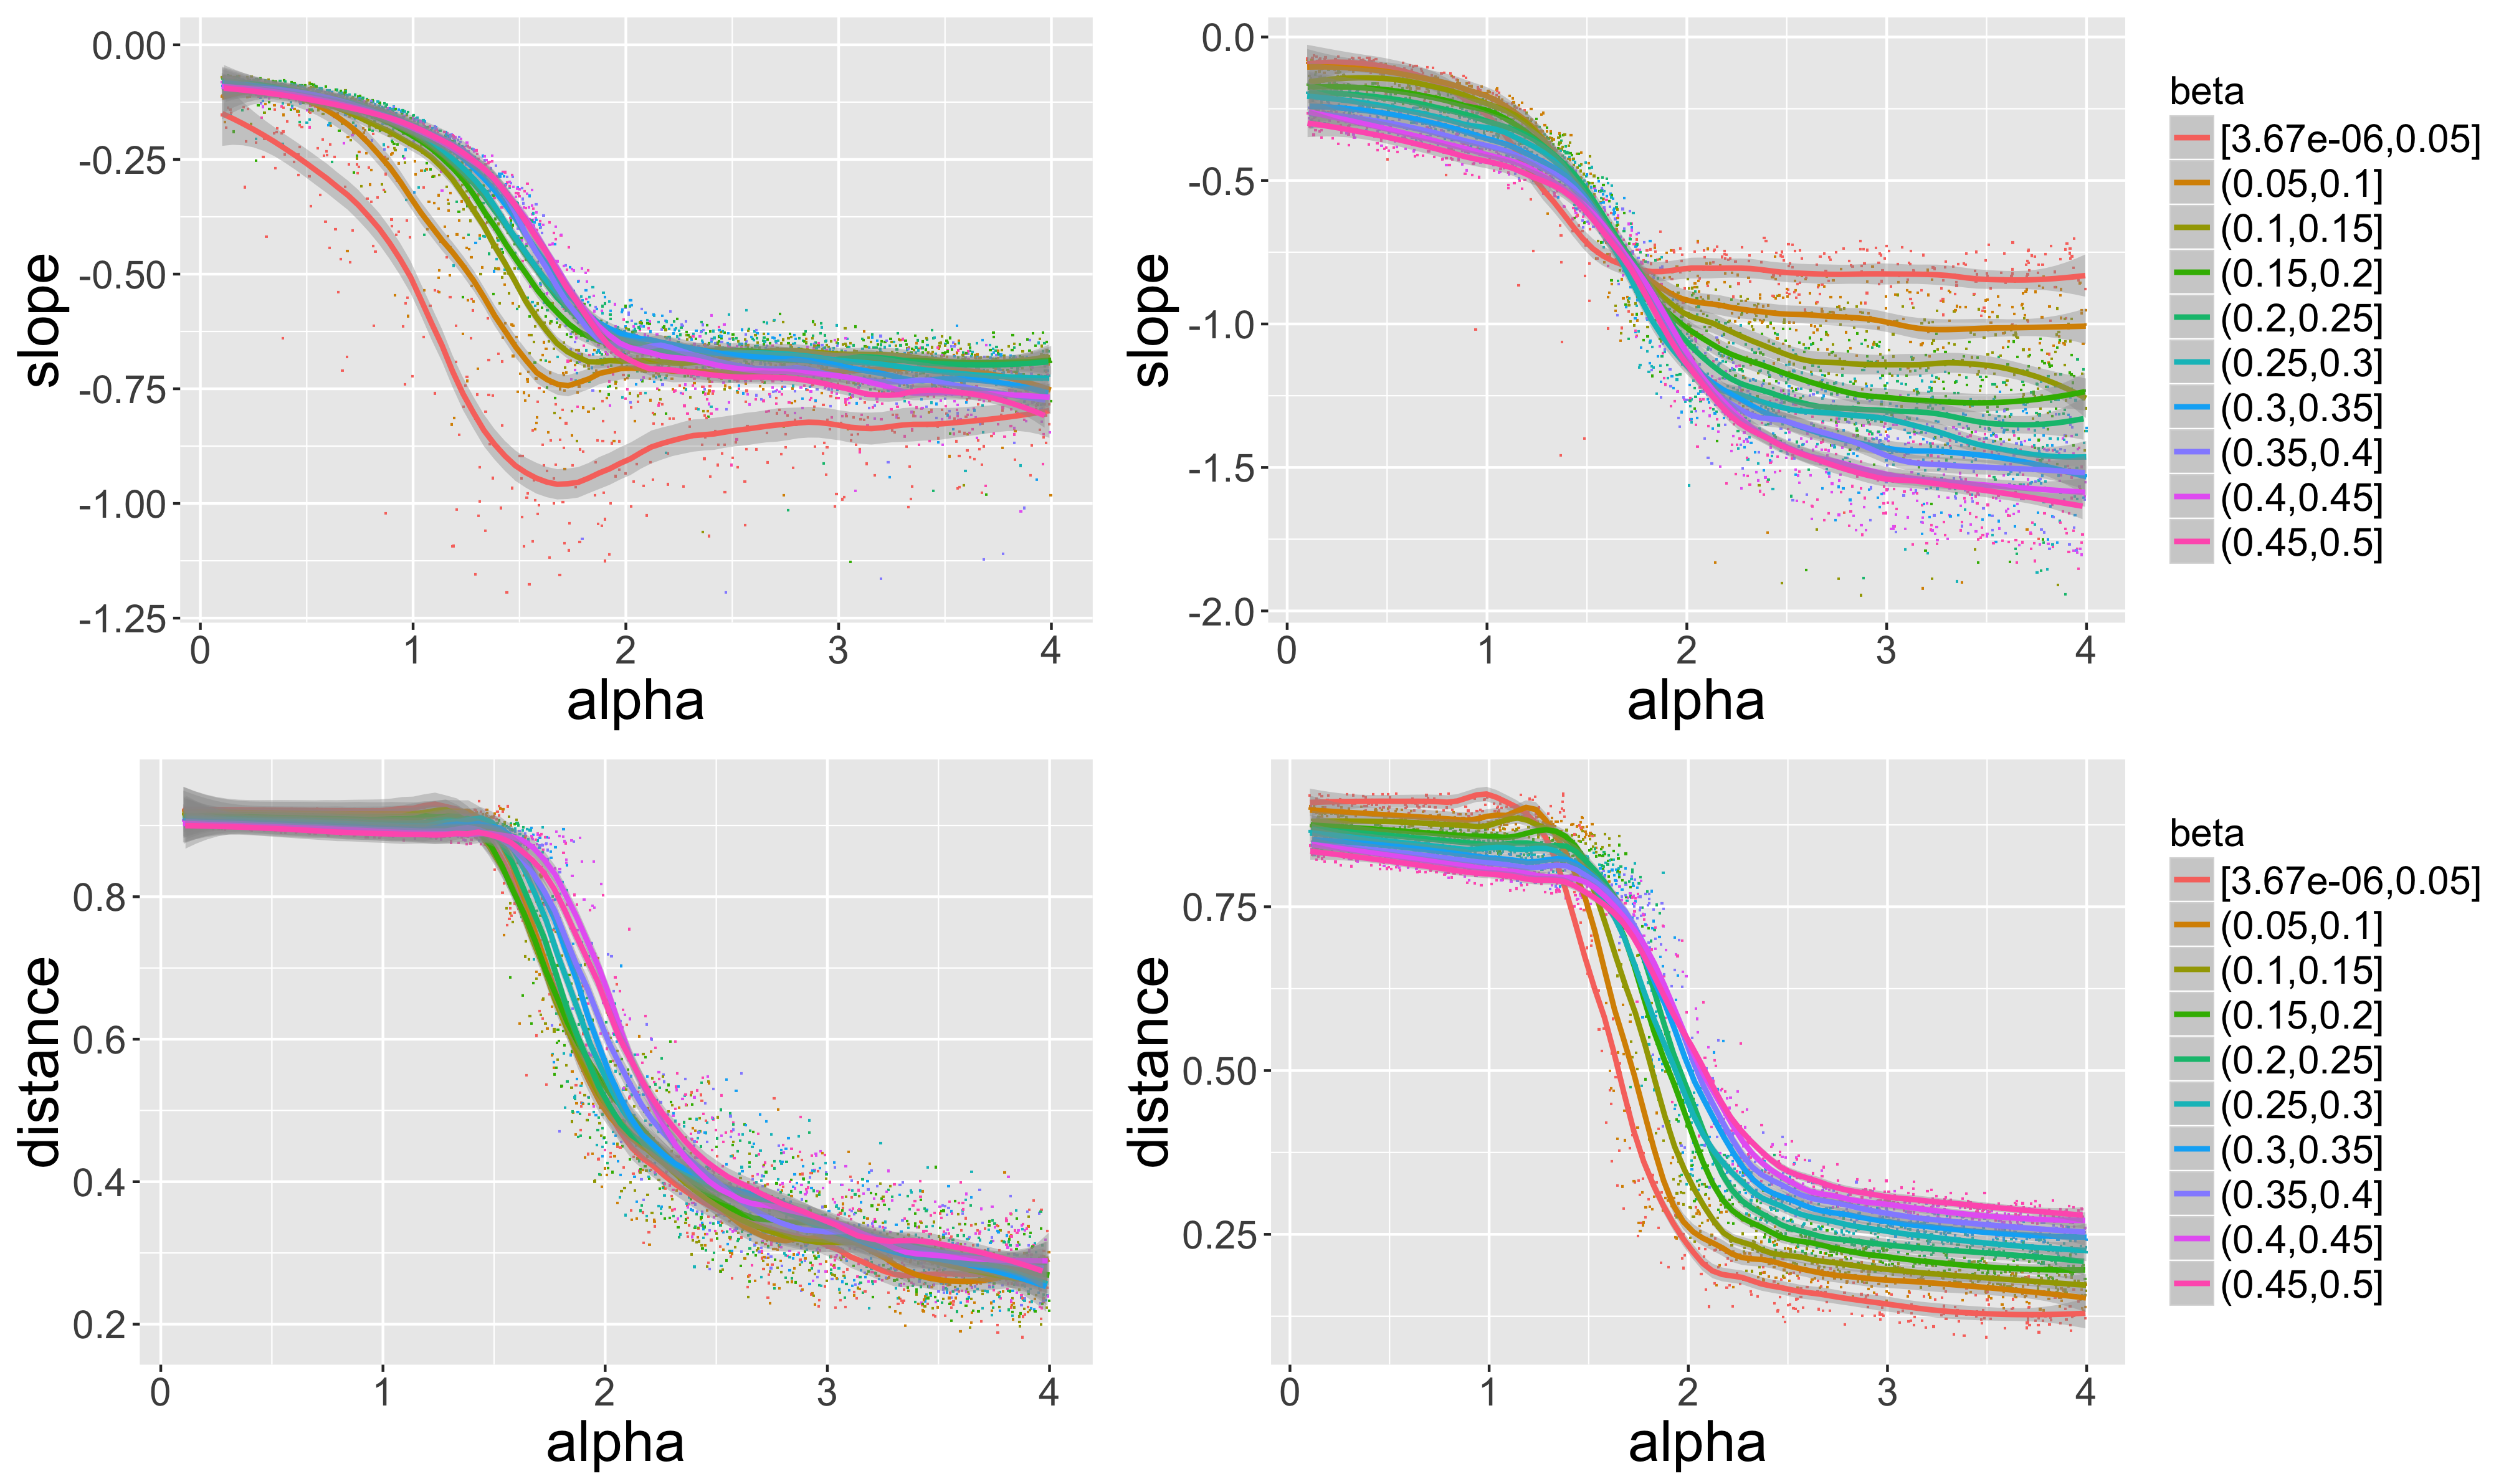
\includegraphics[width=0.9\textwidth]{figures/density_Fig3}

\footnotesize\textit{Phase transitions of indicators unveiled by exploration of the parameter space (80000 parameter points, 10 repetitions each)}

% comment Arnaud : Préciser (dimensionner)

}




\sframe{Path-dependence and frozen accidents}{

\centering

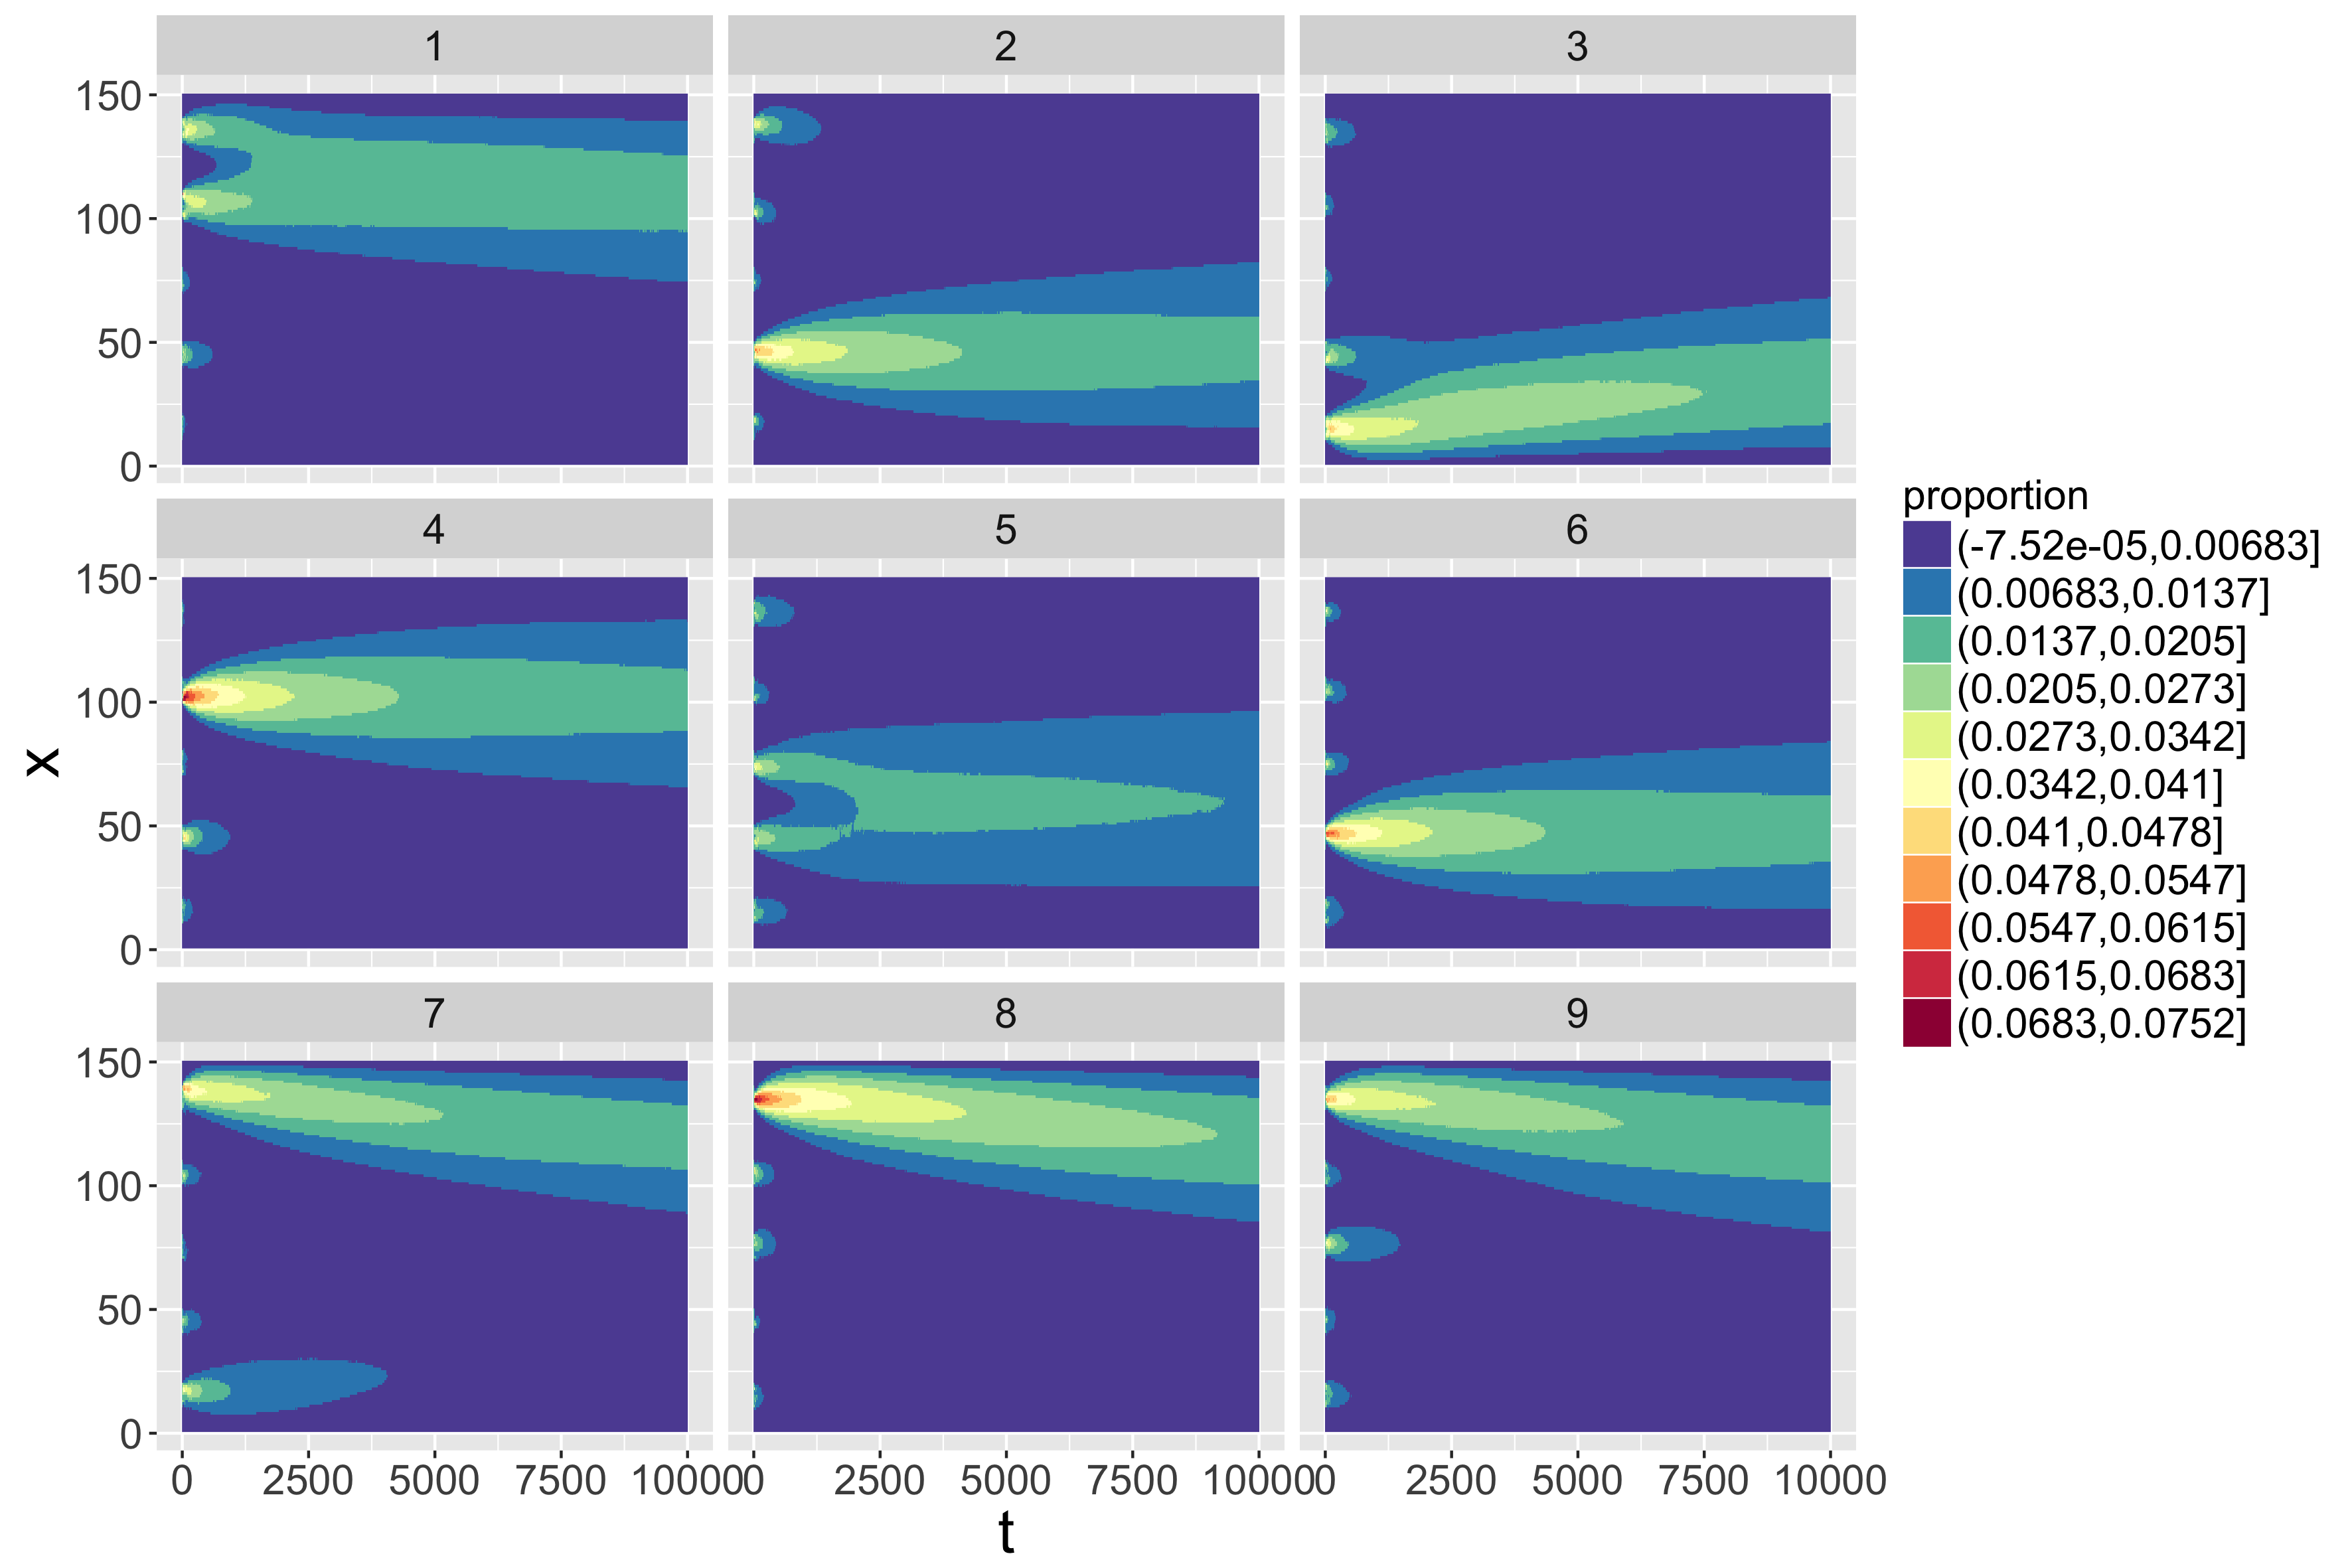
\includegraphics[width=0.8\textwidth]{figures/density_Fig4}

\footnotesize\textit{Illustration of path-dependence in a simplified one-dimensional version of the model: cell trajectories in time for 9 independent repetitions from the same initial configuration.}


}


\sframe{Empirical Data for Calibration}{

% comments Arnaud : Quel lien avec les slides avant et après ? "Real" : le terme me paraît discutable : données empiriques plutôt ?
%  Décrire les données car ici tu passes directement aux indicateurs

\begin{columns}
\column{0.6\textwidth}
\centering
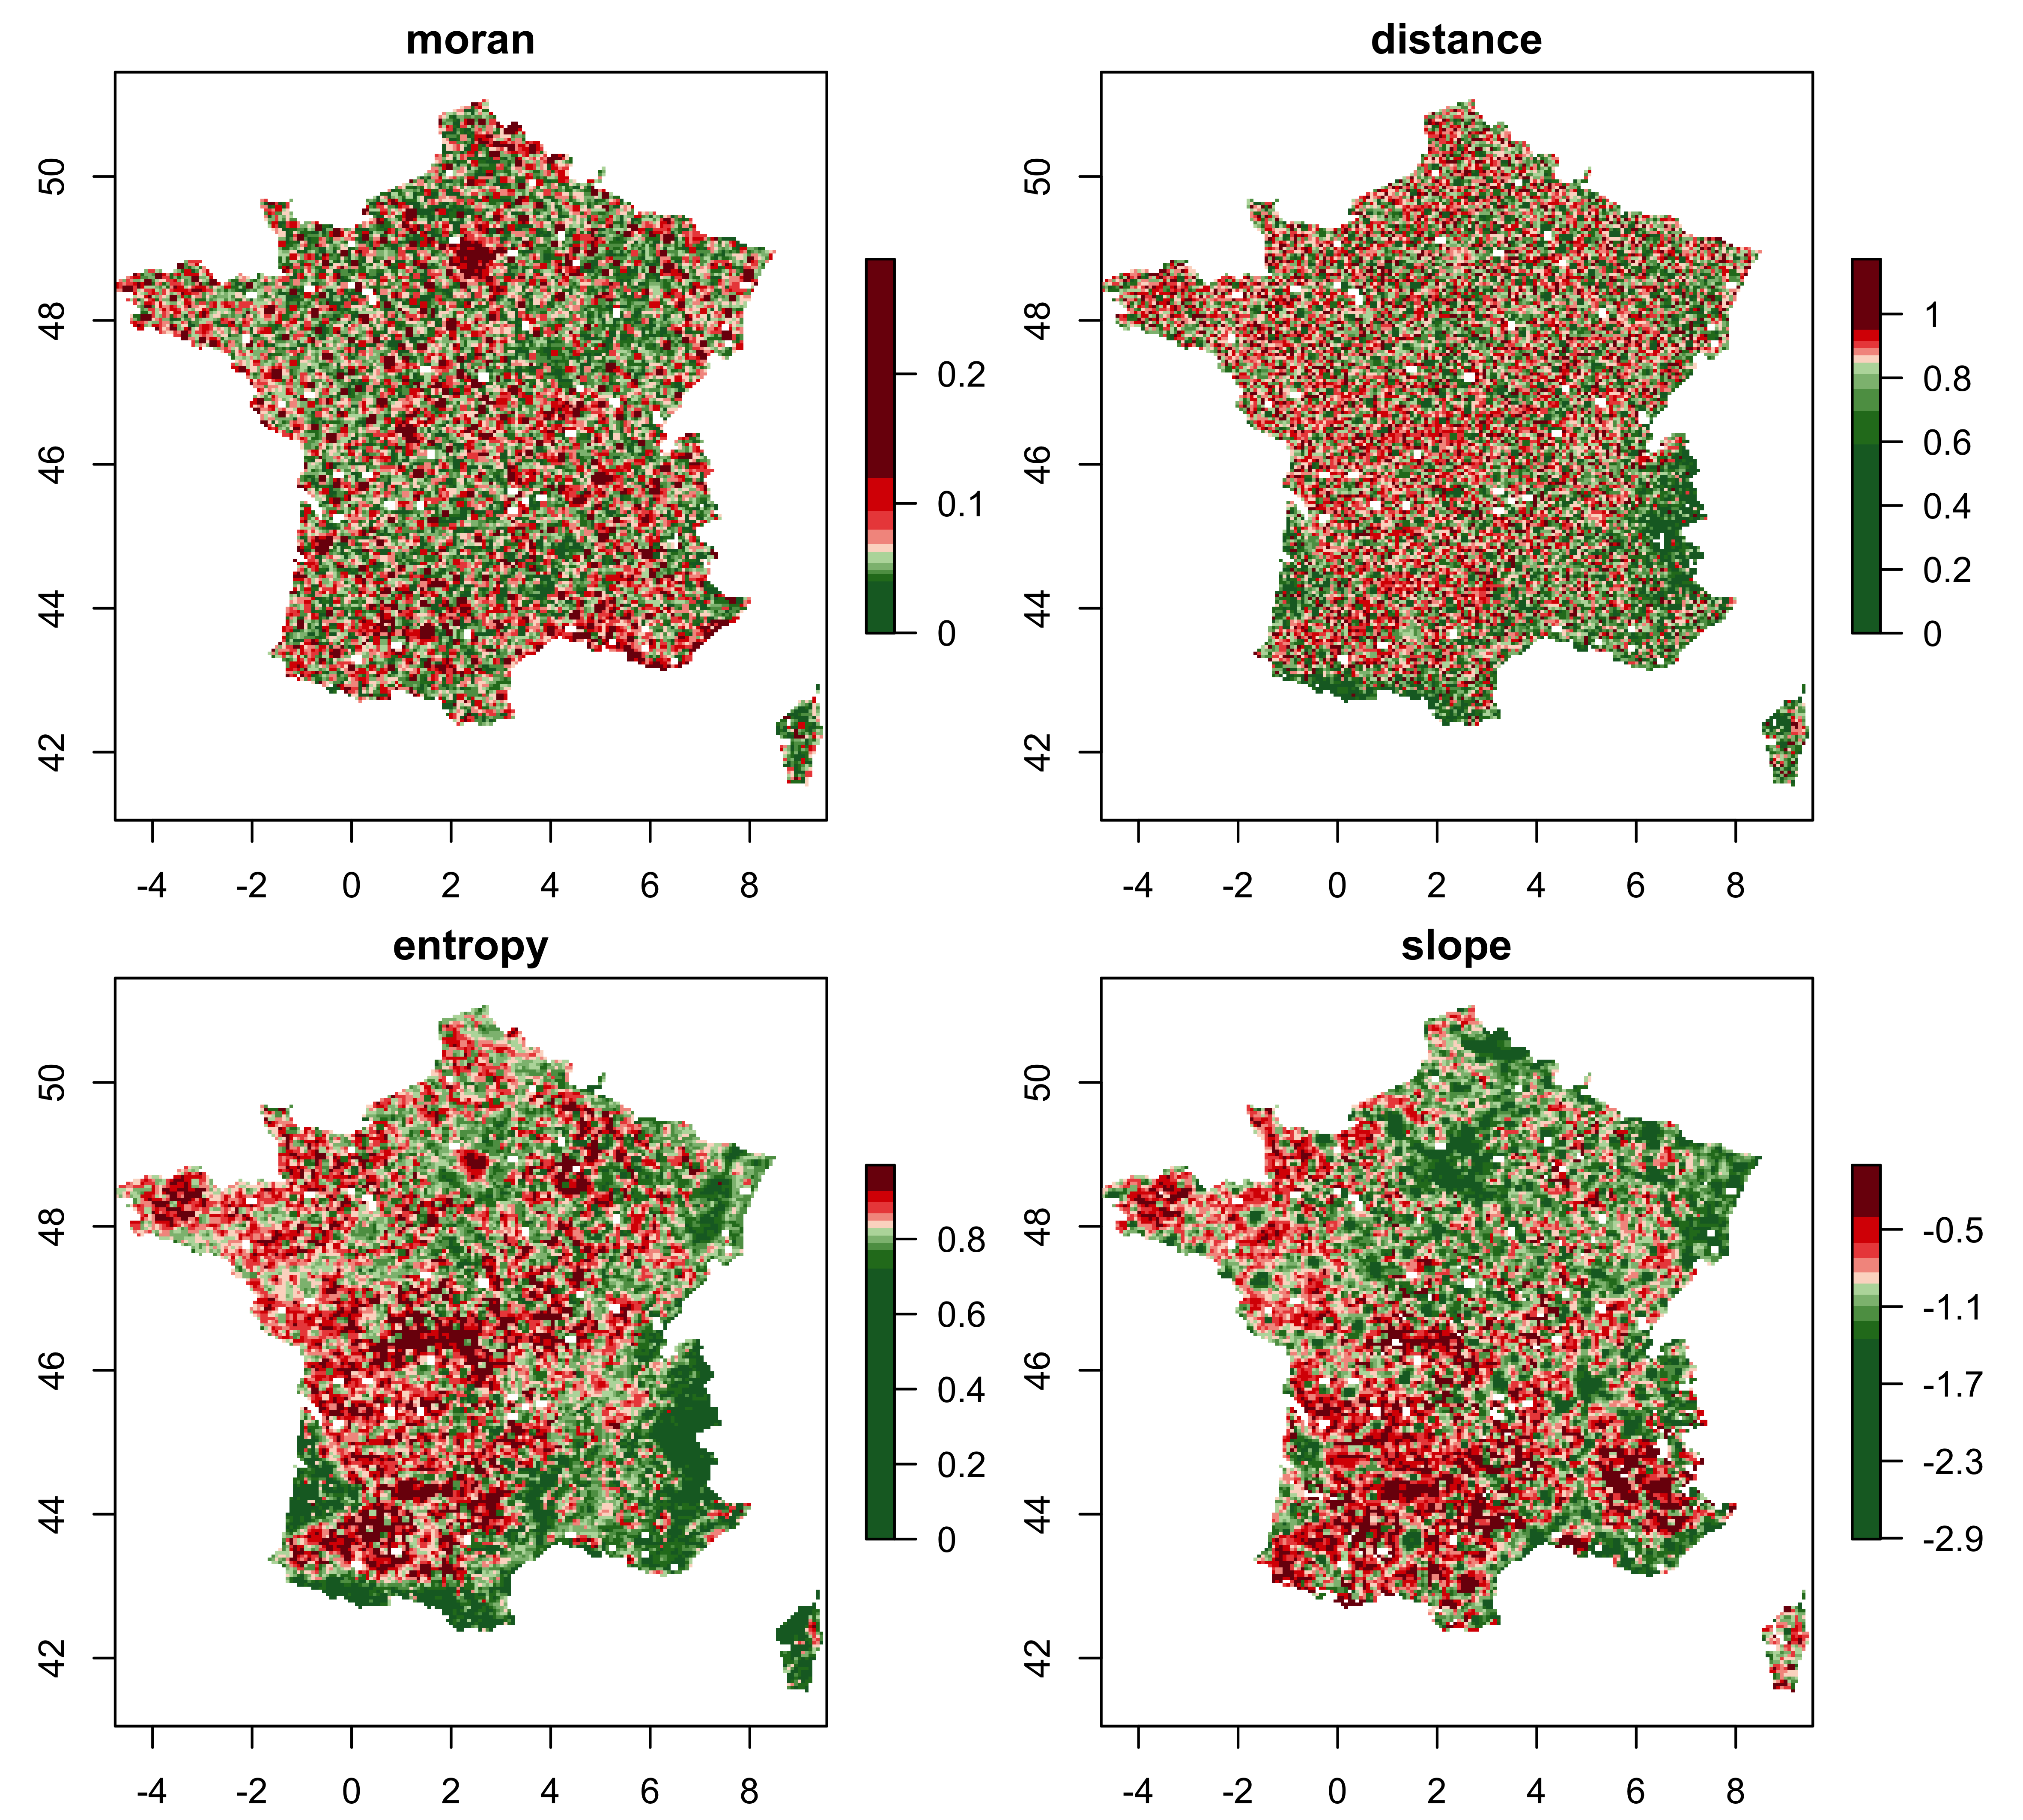
\includegraphics[width=\textwidth]{figures/density_indics_morpho_discrquantiles}
\column{0.3\textwidth}
\centering
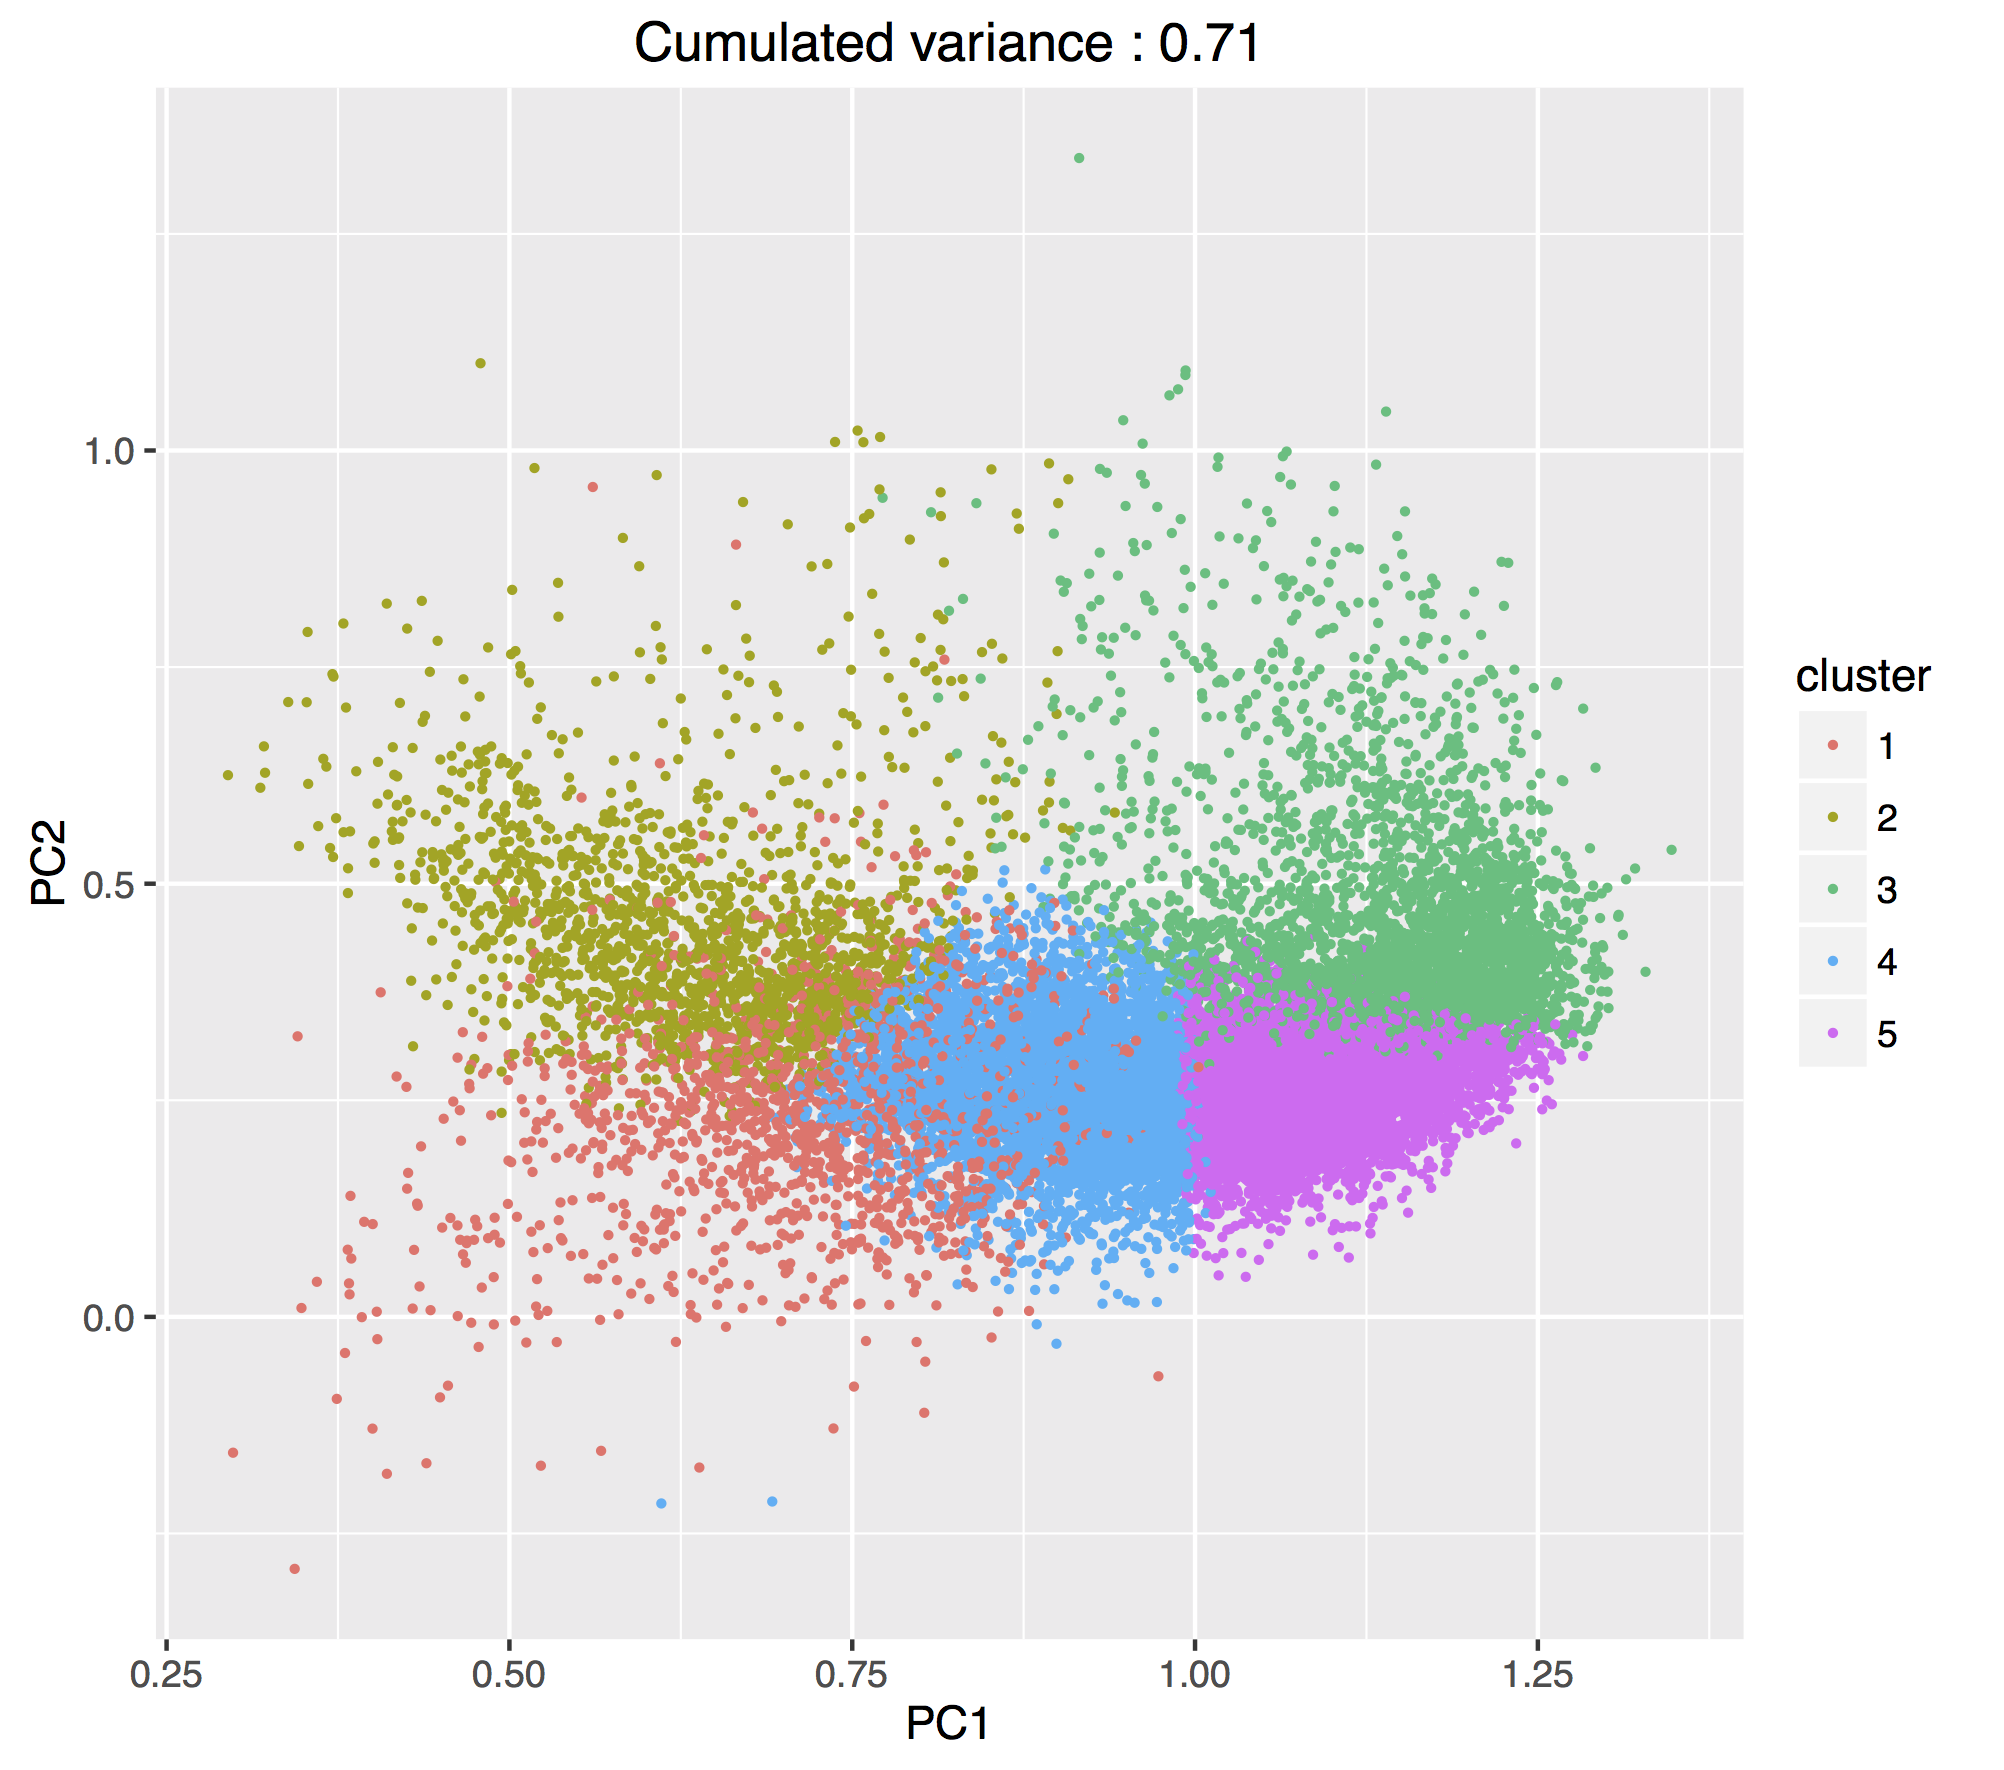
\includegraphics[width=\textwidth]{figures/density_cluster_pca_k5_morpho}\\
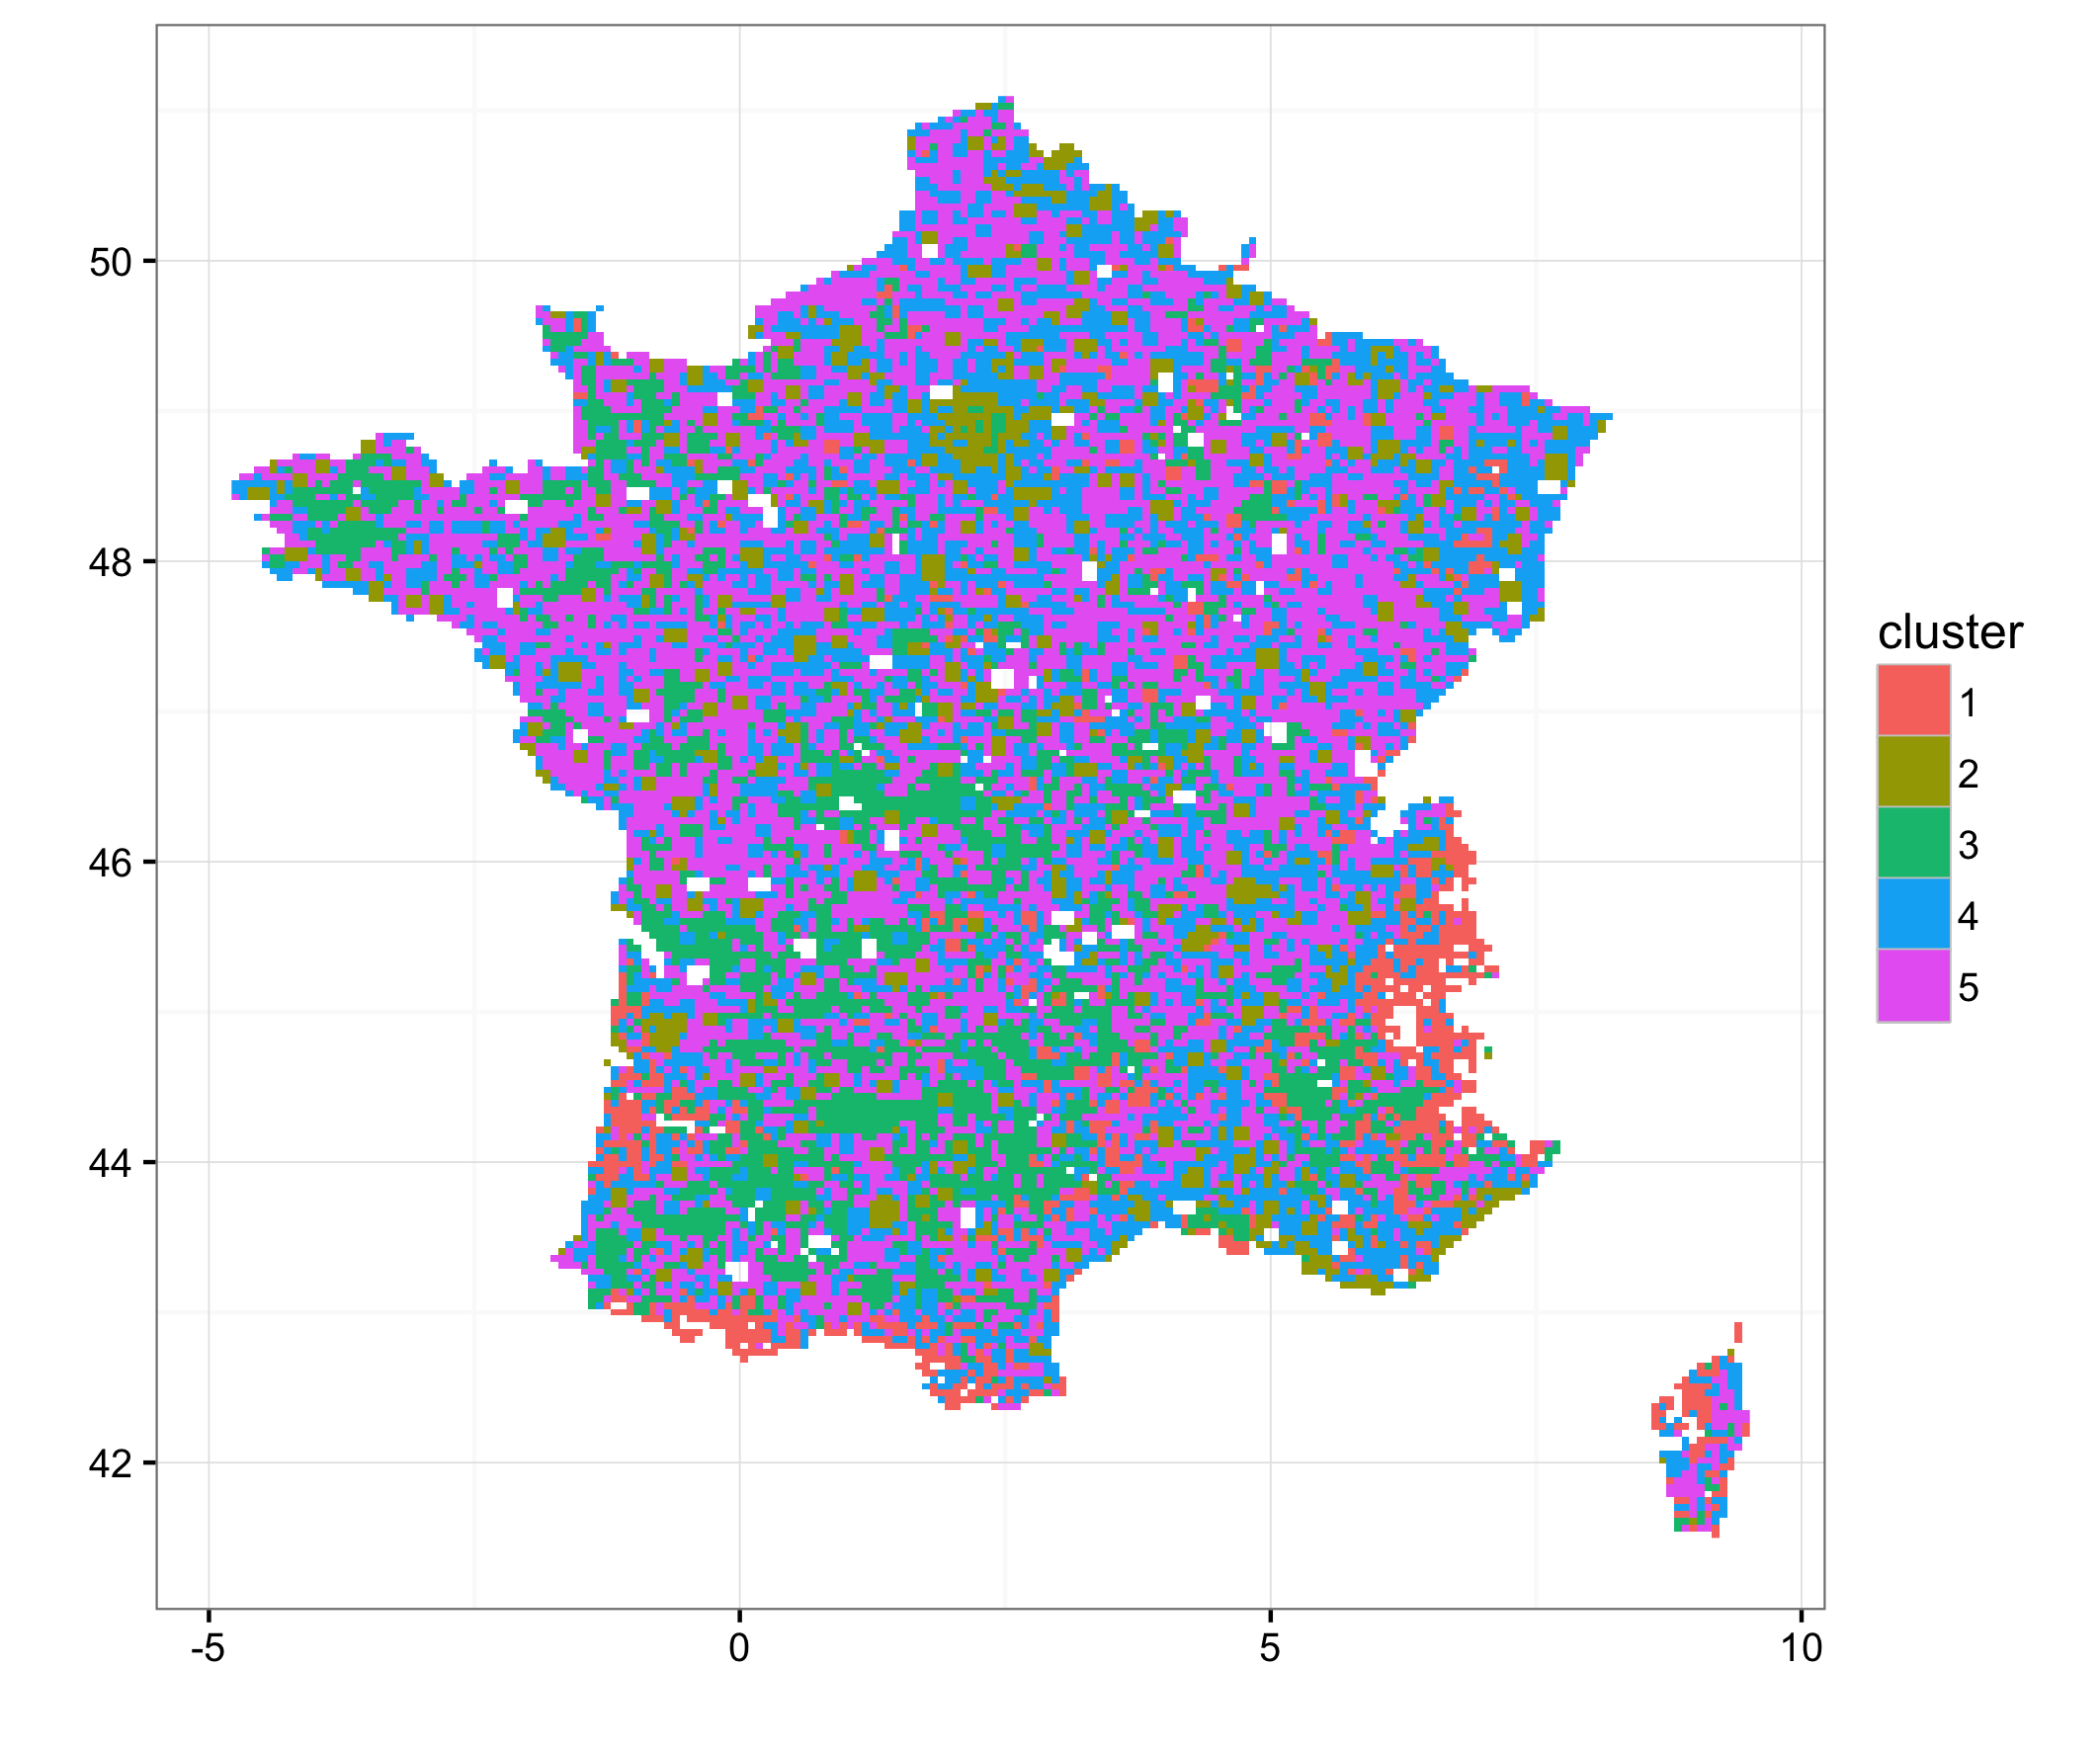
\includegraphics[width=\textwidth]{figures/density_cluster_map_k5_morpho}
\end{columns}

\justify

\footnotesize\textit{Computation of morphological indicators on population density data for Europe (shown here on France), morphological classification.}

}



\sframe{Model Calibration}{

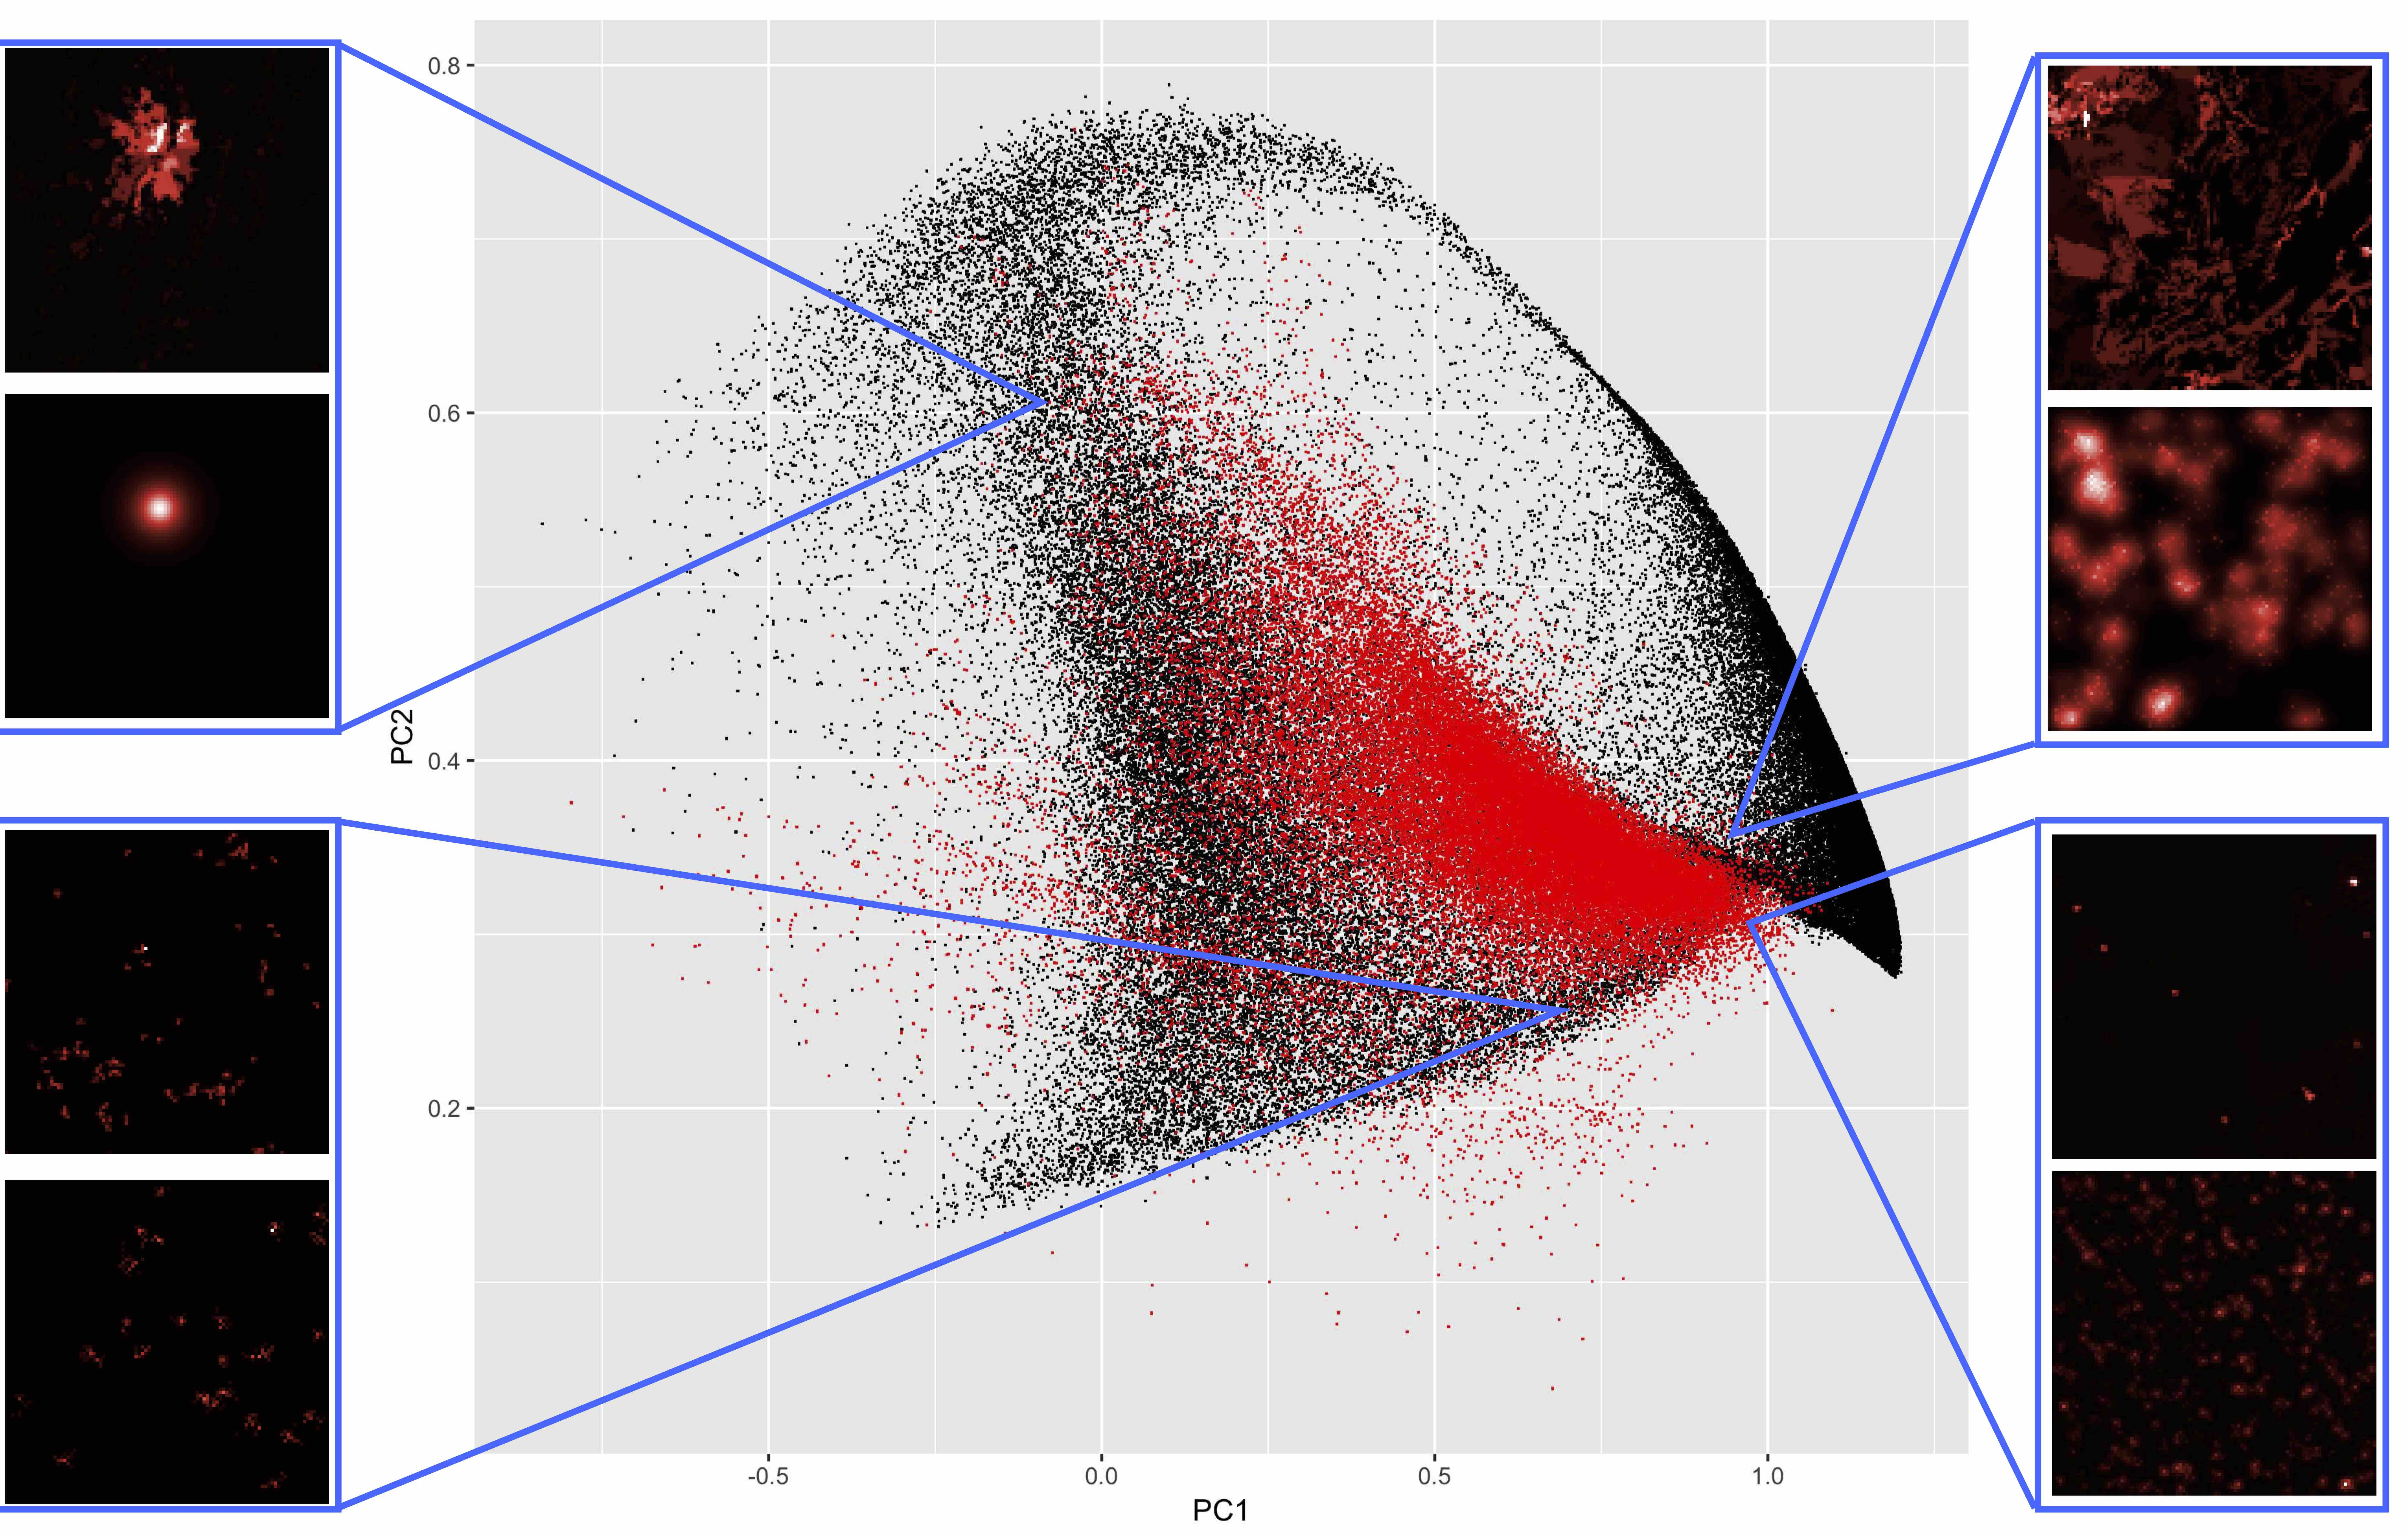
\includegraphics[width=\textwidth]{figures/density_synth}

\footnotesize\textit{Brute force calibration by exploring the parameter space. Reproduction of most existing configuration in the morphological sense (here in principal plan).}

}



\sframe{Model Targeted Exploration}{

\centering

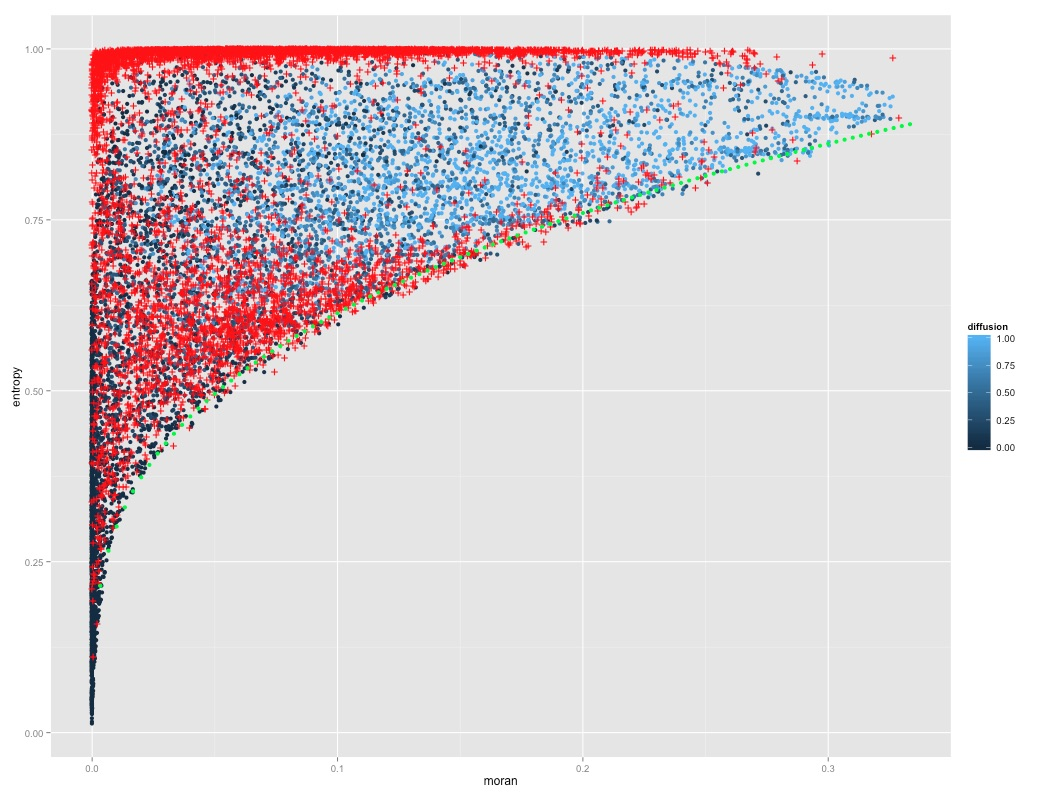
\includegraphics[width=0.8\textwidth]{figures/density_Fig6}

\footnotesize\textit{Potentialities of targeted model explorations: here feasible space using Pattern Space Exploration algorithm \cite{10.1371/journal.pone.0138212}.}

}




\sframe{Including more complex processes ?}{

% transition : representation of territories

\textit{Which ontology to include more complex functional properties ?}

\medskip

$\rightarrow$ Territorial systems as the strong coupling between territories and (potential and realized) networks \cite{dupuy1987vers}.

\medskip

$\rightarrow$ Networks convey functional notions of centralities and accessibility, among others ; have furthermore proper topological properties.


}


\sframe{Interactions between Networks and Territories}{

% qualitative slide
% eventually layus on literature with the cit nw ? maybe too much
% def. covevol : besoin coevol regimes, annexe
% idem macrocoevol en annexe


\textit{Complex co-evolutive processes between Territories and Transportation Networks}

\medskip

\centering

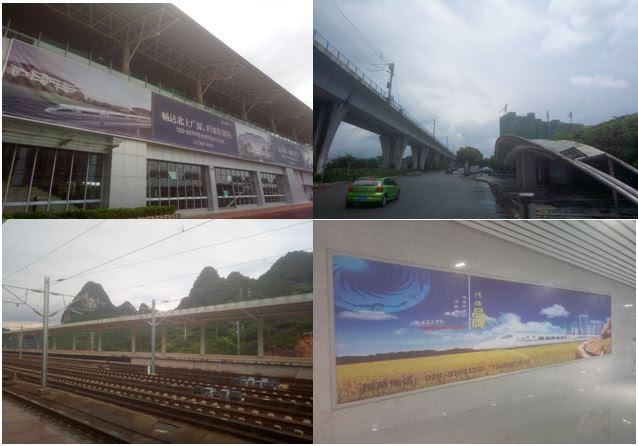
\includegraphics[height=0.7\textheight]{figures/intro_fieldwork}

\footnotesize

\textit{Expanding HSR network in China and ambiguous effects (Source : fieldwork survey)}


}









%%%%%%%%%%%%%%%
%%%% RBD model

\sframe{A basic hybrid model}{


\begin{itemize}

\item \begin{justify}What is the influence of proximity on urban form? Proposition of modeling transportation
network coupled with a Cellular Automaton in \cite{moreno2007conception,MBB09}.\end{justify}

\item \begin{justify}We generalize and extend this model: from morphological to functional
properties of the urban environment. We couple a Cellular Automaton with an evolving network.\\
\textbf{Research question:} \textit{Is it possible to reproduce patterns of urban form with a model of urban development taking into account both transportation network and city scape, including form and function ?}\end{justify}

\item \begin{justify}Our objective is to apply the model to a real case, by proposing a method for
the optimization of planning on all possible functional configurations.
\end{justify}

\end{itemize}



}



\sframe{Model description : settings and agents}{
\vfill{}

\begin{itemize}
\item Fixed agents: cells in a square lattice $(L_{i,j})_{1\leq i,j\leq N}$
, occupied or not (function \textrm{$\ensuremath{\delta(i,j,t)\in\{0,1\}}$)}
\end{itemize}
\vfill{}

\begin{itemize}
\item Evolving euclidian network $G(t)=(V(t),E(t))$,
including fixed city centers $C_{0}\subset V(0)$ for each an activity
$a\in\{1,\ldots,a_{max}\}$ is defined (functional properties of the
urban scape).
\end{itemize}
\vfill{}

\begin{itemize}
\item Heterogeneous explicative variables $(d_{k})_{1\leq k\leq K}$ defined
on cells, with associated weights $(\alpha_{k})_{1\leq k\leq K}$
(main parameters of the model), that are:

\begin{itemize}
\item $d_{1}$ the density around the cell (in a fixed radius $r$)
\item $d_{2}$ the distance to the nearest road
\item $d_{3}$ the distance to the nearest town center through the network
\item \textrm{$d_{4}(i,j,t)=\left(\frac{1}{a_{\max}}\sum_{a=1}^{a_{\max}}d_{3}(i,j,t;a)^{p_{4}}\right)^{1/p_{4}}$
}: integrated accessibility of activities
\end{itemize}
\end{itemize}
\vfill{}
}



\sframe{Model workflow}{

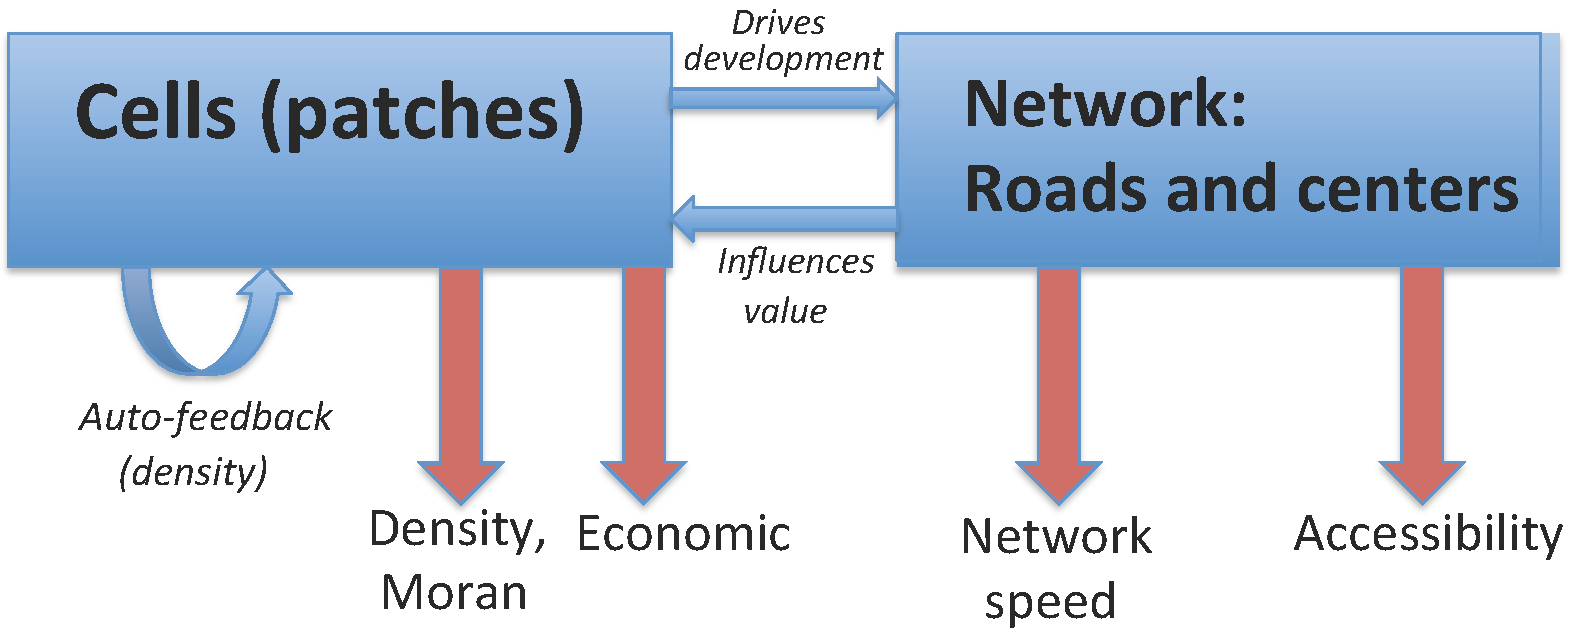
\includegraphics[scale=0.30]{figures/rbd_flowchart.png}

}




\sframe{Evolution rules}{

At each time step:\vfill{}

\begin{itemize}
\item Sprawling of occupied urban structure. The best $N$ cells according
to the value $v(i,j,t)=\frac{1}{\sum_{k}\alpha_{k}}\sum_{k=1}^{K}\alpha_{k}\;\frac{d_{k,\max}(t)-d_{k}(i,j,t)}{d_{k,\max}(t)-d_{k,\min}(t)}$
are built.\vfill{}

\item Adaptation of the network: when a new cell is built, if $d_{2}>\theta_{2}$, the cell is connected to the network by a new perpendicular
road.\vfill{}

\end{itemize}
}


\sframe{Evaluation functions}{

\textit{\Large Objective Morphological indicators}{\Large \par}
\begin{itemize}
\item Integrated local density $ $$D(t)=\left(\frac{1}{\sum_{i,j}\delta(i,j,t)}\!\!\sum_{{\scriptstyle {i,j=1\atop {\scriptstyle \delta(i,j,t)\neq0}}}}^{N}\!\! d_{1}(i,j,t)^{p_{D}}\right)^{1/p_{D}}$
\item Moran index (``polycentric'' character of a distribution of populated
cells, \cite{tsai2005quantifying,lenechet:hal-00696445}): world decomposed
in a grid of size $M$ ($1\ll M\ll N$ ), $(P_{i})_{1\leq i\leq M}$
are populations in each part of the grid, then
\[
I(t)=\frac{M^{2}}{\sum_{\mu\neq\nu}1/d_{\mu\nu}}\frac{\sum_{\mu\neq\nu}(P_{\mu}-\overline{P})(P_{\nu}-\overline{P})/d_{\mu\nu}}{\sum_{\mu=1}^{M^{2}}(P_{\mu}-\overline{P})^{2}}
\]

\end{itemize}

}



\sframe{Evaluation functions}{

\textit{\Large Performance indicators}{\Large \par}
\begin{itemize}
\item Network speed (\cite{banos2012towards}) $S(t)=\left(\frac{1}{\sum_{i,j}\delta(i,j,t)}\!\!\sum_{{\scriptstyle {i,j=1\atop {\scriptstyle \delta(i,j,t)\neq0}}}}^{N}\!\!\left(\frac{d_{3}(i,j,t)}{e_{3}(i,j,t)}\right)^{p_{S}}\right)^{1/p_{S}}$
with $e_{3}(i,j,t)$ euclidian distance to nearest center
\item Normalized functional accessibility $A(t)=\left(\frac{1}{\sum_{i,j}\delta(i,j,t)}\!\!\sum_{{\scriptstyle {i,j=1\atop {\scriptstyle \delta(i,j,t)\neq0}}}}^{N}\!\!\left(\frac{d_{4}(i,j,t)}{d_{4,\max}(t)}\right)^{p_{A}}\right)^{1/p_{A}}$
\item Socio-economic segregation potential: run on the generated configuration
of an economic residential ABM dynamics (\cite{schelling1969models},
\cite{benenson1998multi}), which is strongly sensitive to spatial structure
according to \cite{banos2012network}, calculation of the final spatialized
segregation index $E$.
\end{itemize}

}



\sframe{Examples of generated shapes}{

%%manually reset sub float counter (why does it not ?)
\setcounter{subfigure}{0}

\begin{figure}
\hspace*{-1cm}
\subfloat[``A city can be a tree'', \cite{alexander1964city}]{
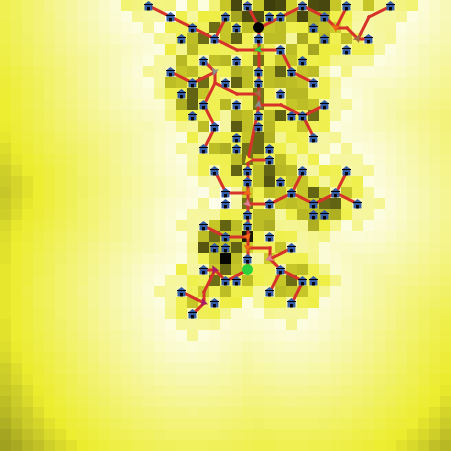
\includegraphics[scale=0.25]{figures/rbd_TreeLikeCity}}
\subfloat[Intermediate shape]{
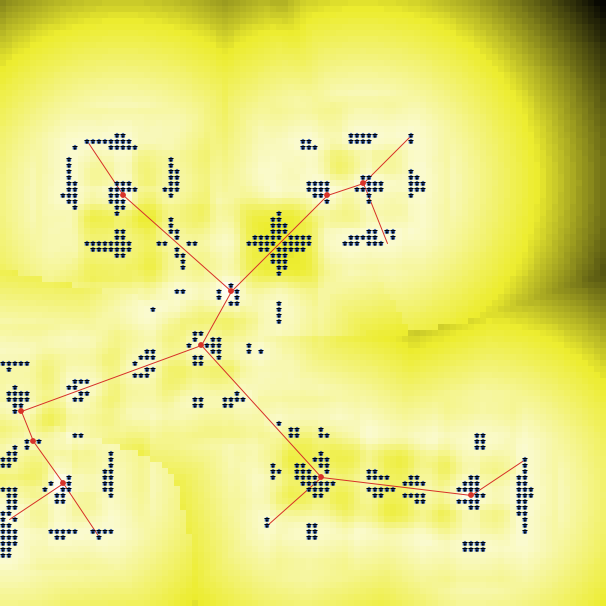
\includegraphics[scale=0.19]{figures/rbd_LinkedCenters_eqCoefs_MoreCells}}
\subfloat[One center, no density]{
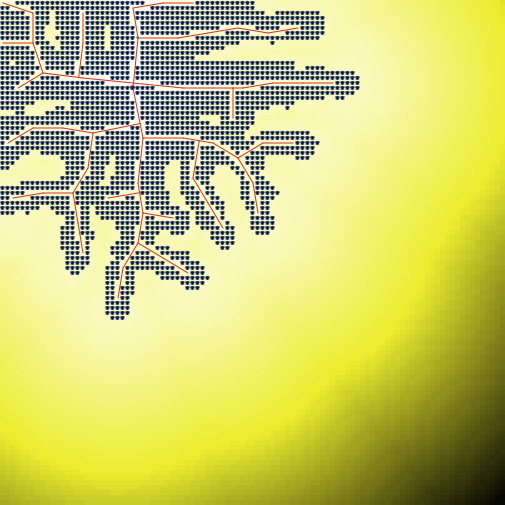
\includegraphics[scale=0.23]{figures/rbd_bigWorld-distances}}
\end{figure}


}


\sframe{Typology of structures}{

\begin{columns}[c]

\column{5.5cm}

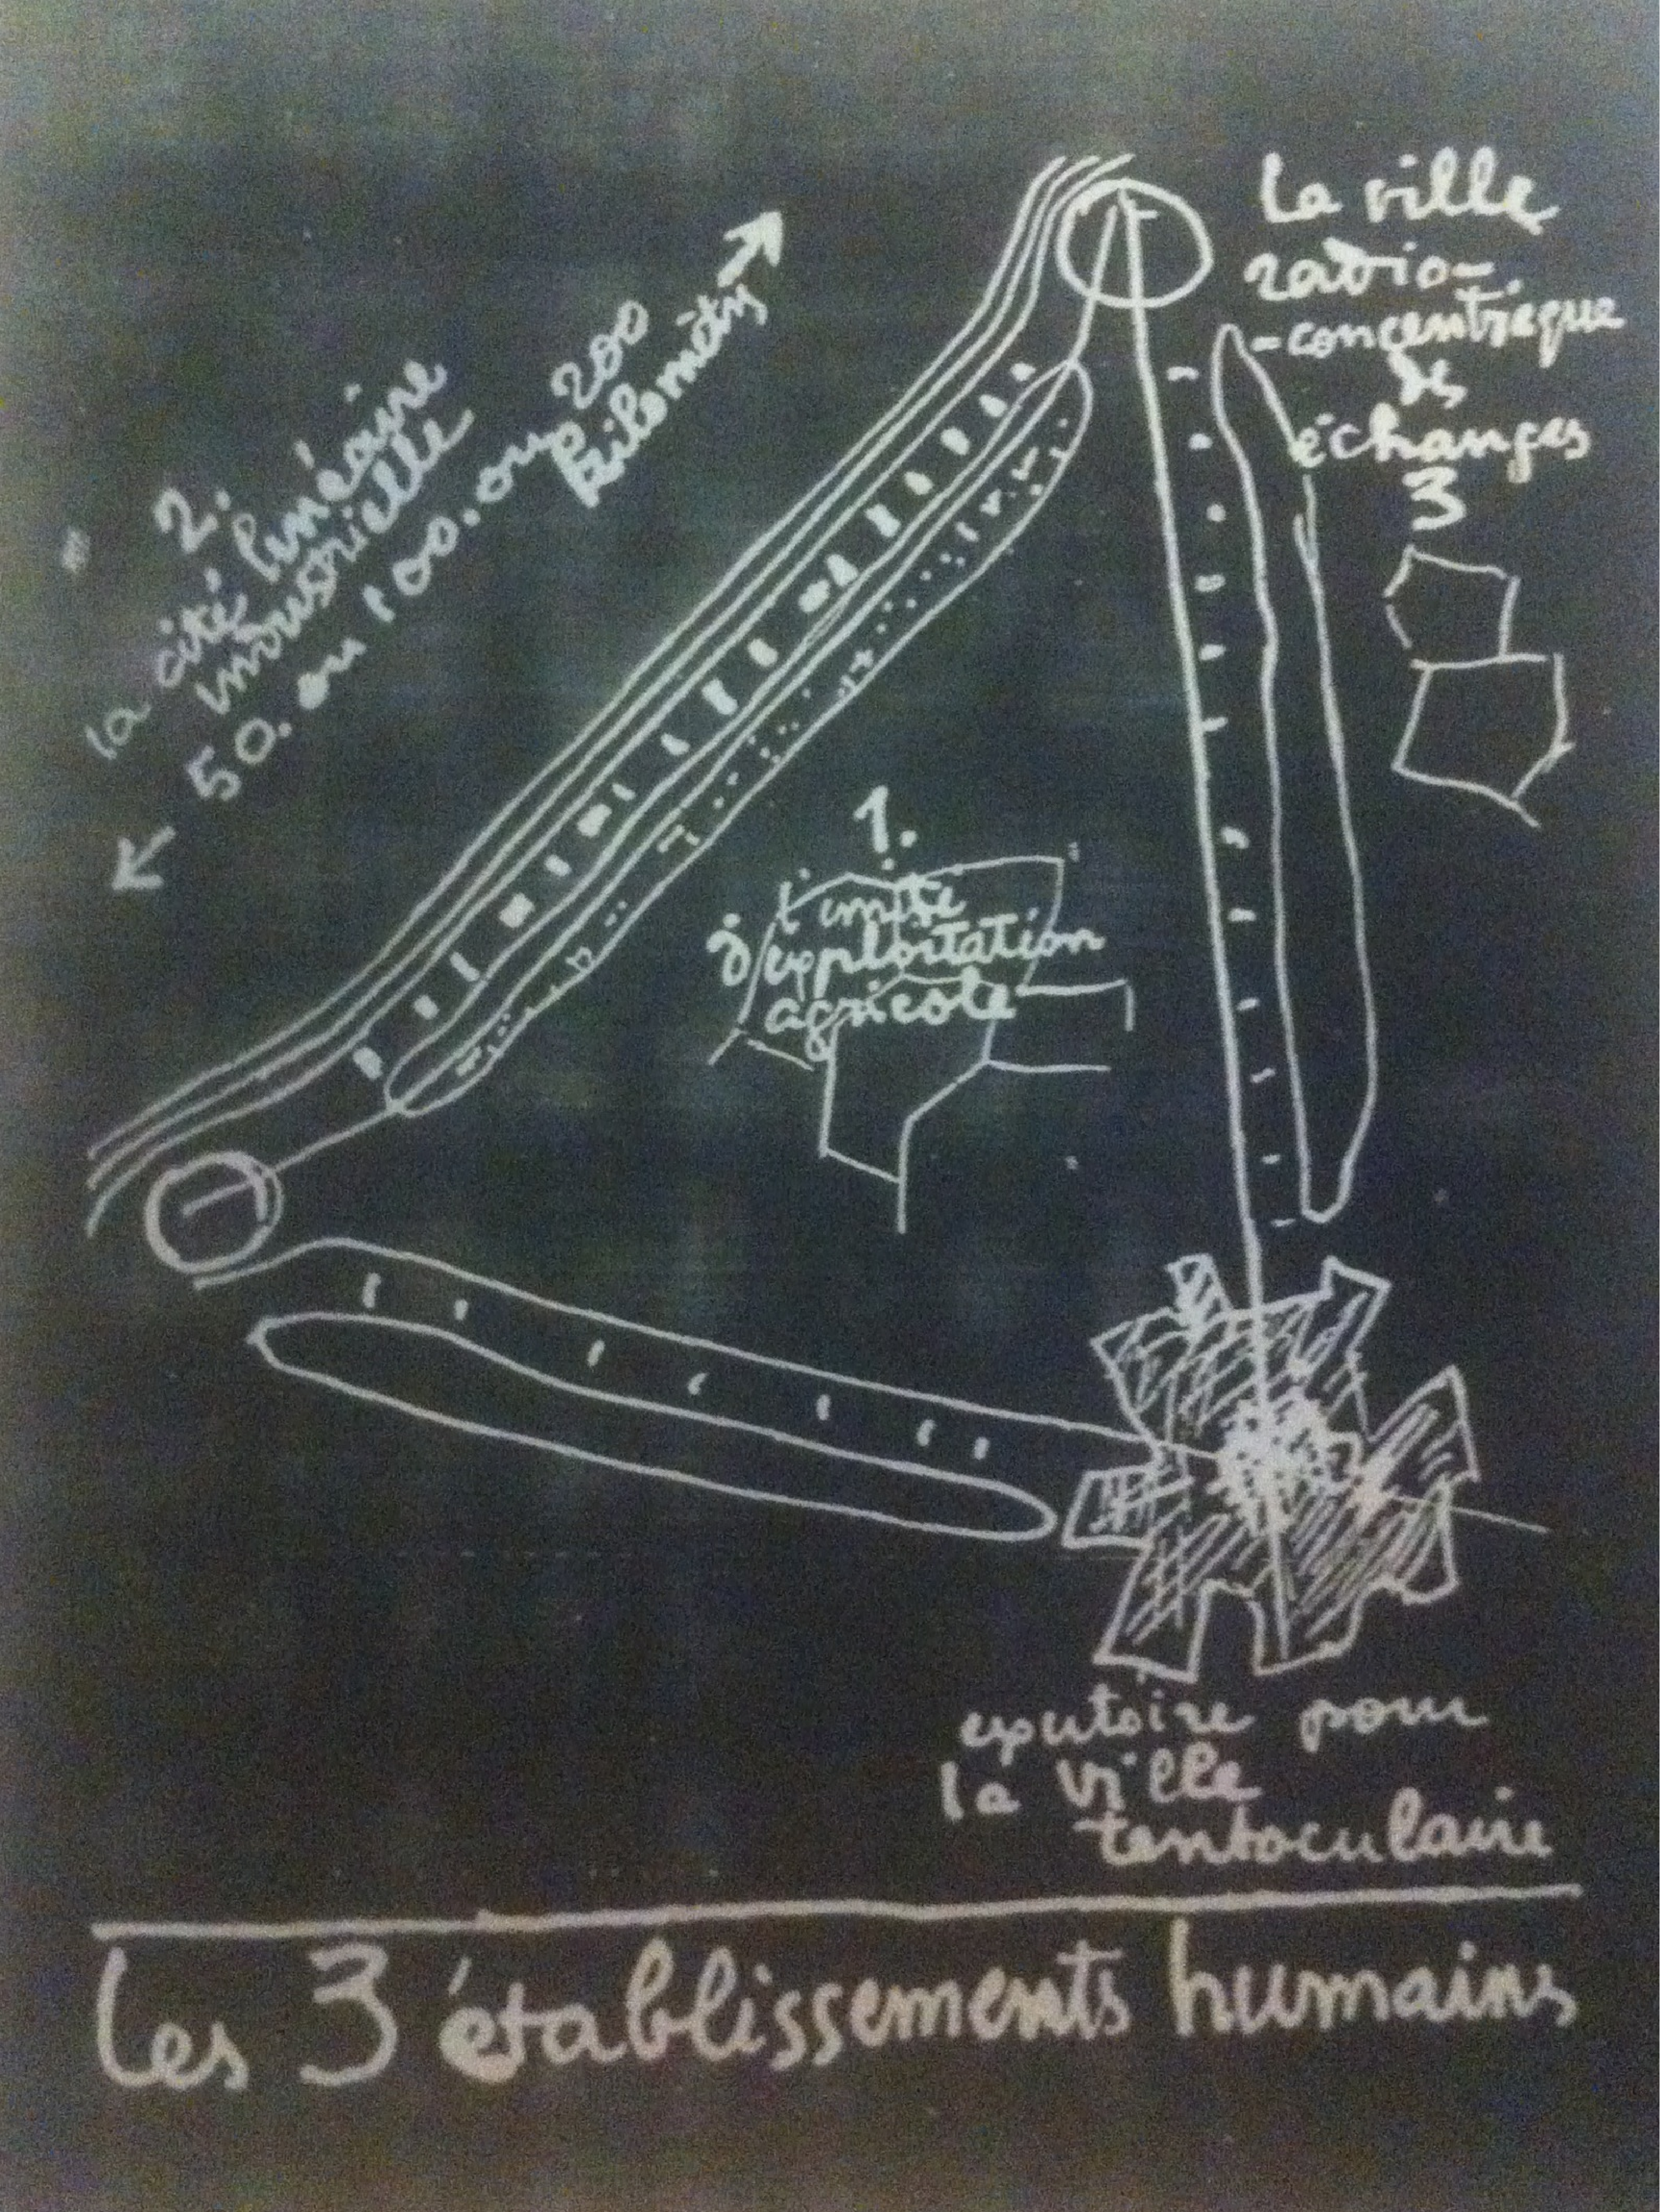
\includegraphics[trim=0cm 0cm 2cm 0cm,width=0.8\textwidth]{figures/rbd_CorbuEtablissements}


\column{3cm}
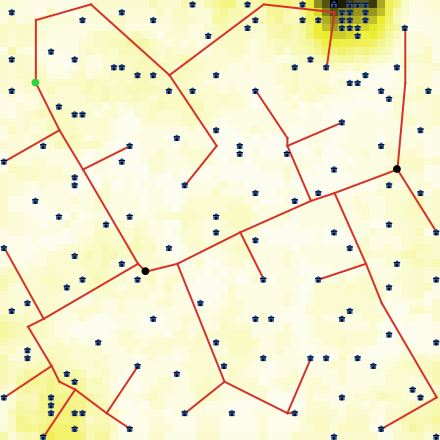
\includegraphics[width=0.92\textwidth]{figures/rbd_corbuDensity}\\
\vspace{0.3cm}
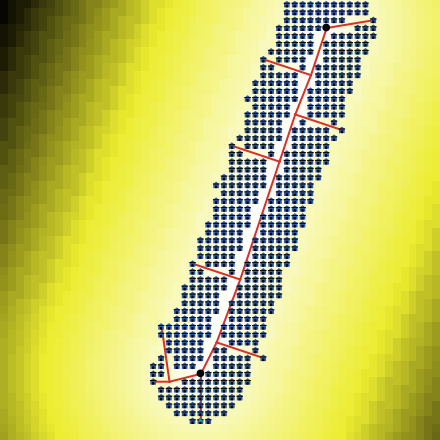
\includegraphics[width=0.92\textwidth]{figures/rbd_corbuLinearCiudad}

\column{3cm}
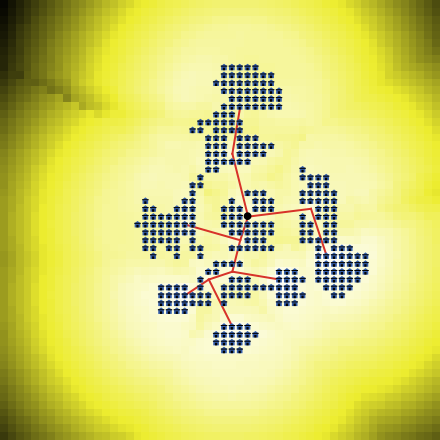
\includegraphics[width=1\textwidth]{figures/rbd_corbuRadiant}


\end{columns}


\textit{Parallel between Le Corbusier's typology of ``human settlements''
and some generated structures}

}


\sframe{Morphological classification}{

\begin{columns}
\column{7.5cm}
\begin{figure}
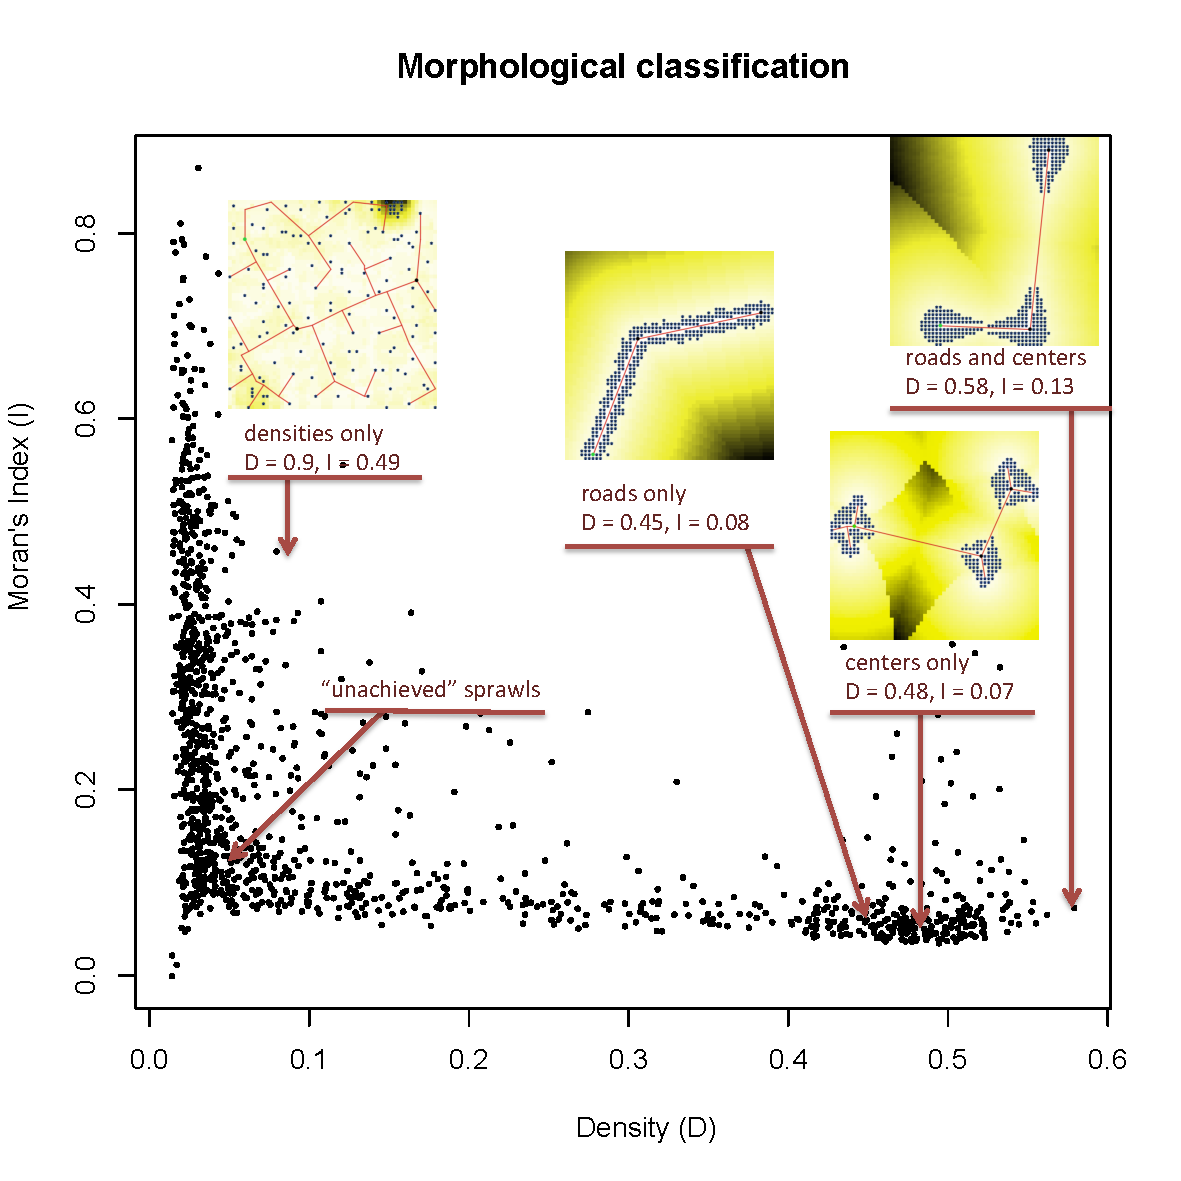
\includegraphics[trim=0cm 0cm 0cm 1.7cm,width=1\textwidth]{figures/rbd_morpho}
\end{figure}

\column{4cm}
\textit{Projection in the morphological plane of indicators; classification
of some structures.}

\end{columns}

}




\sframe{Statistical analysis}{

\begin{centercolumns}%{}


\column{5cm}


\begin{figure}
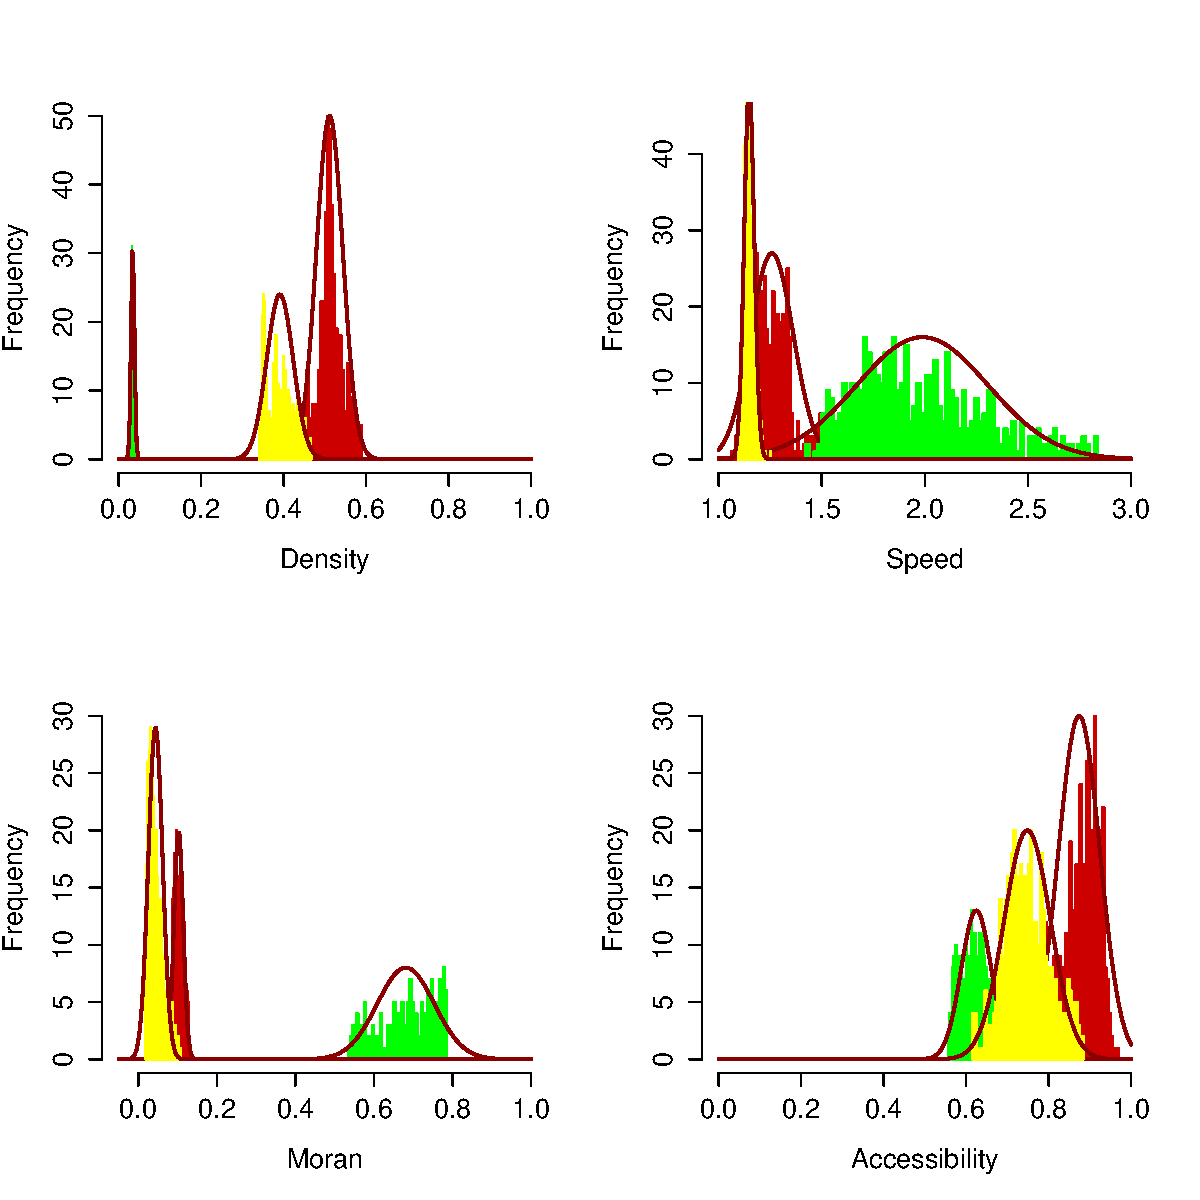
\includegraphics[trim=1cm 1cm 3cm 2cm,width=1\textwidth]{figures/rbd_goodHists2}
\end{figure}

\column{6cm}


\textit{Statistical distributions of outputs for different points in parameter
space.}


\begin{itemize}
\item Statistical study of the behavior of the model: is the output sensitive
to initial spatial configurations?

\item Internal robustness of the model

\item Number of repetitions needed : $\ensuremath{n=(2\sigma\!\cdot\!1.96/0.05)^{2}\simeq60}$
repetitions for 95\% confidence interval of width 0.05
\end{itemize}
\end{centercolumns}

}


\sframe{Exploration of the parameter space}{
\begin{columns}

\column{6cm}


\begin{figure}
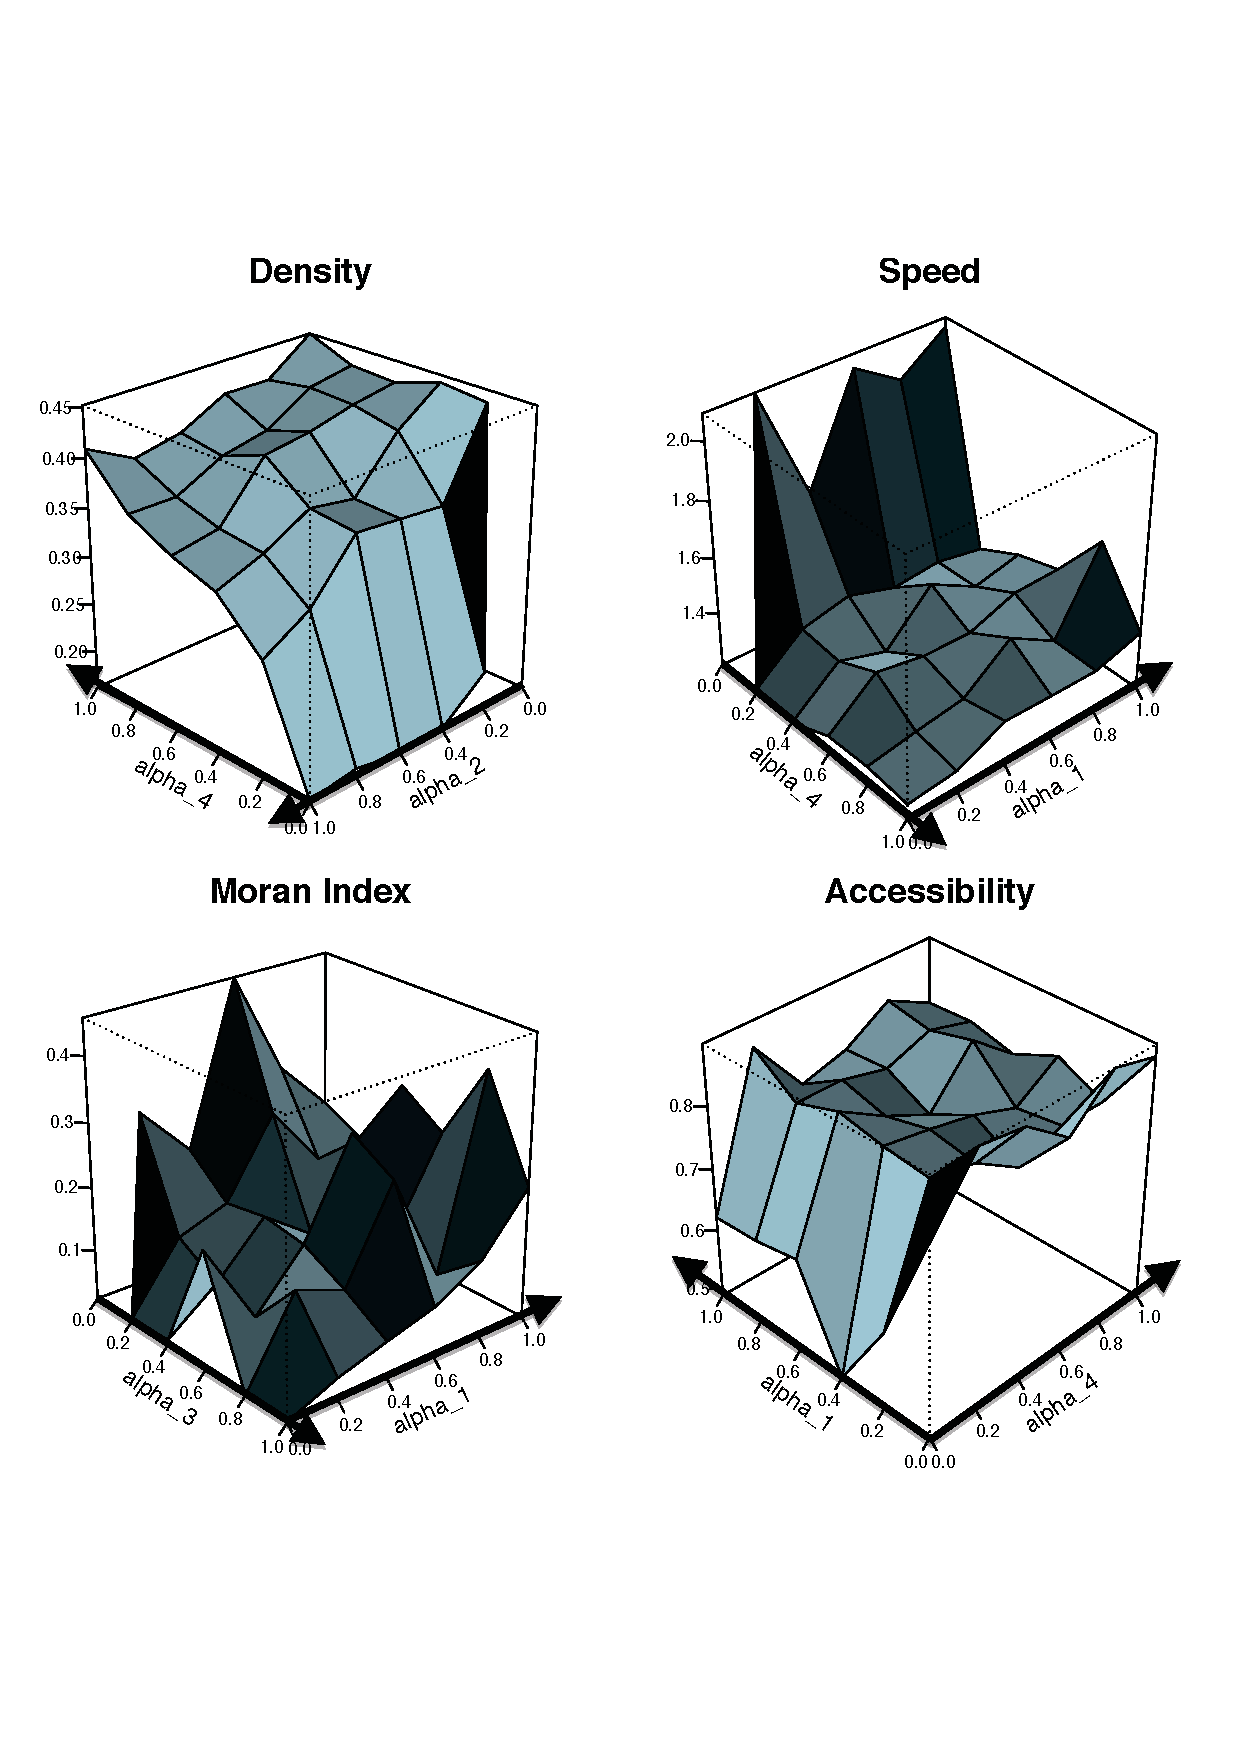
\includegraphics[trim=1cm 4cm 1cm 7cm,width=1.1\textwidth]{figures/rbd_3DWithArrowsLast}
\end{figure}

\column{5cm}

\textit{Sample surface plots of the evaluation functions.}


\begin{itemize}
\item Finer exploration of the $(\alpha_{k})$ parameter space: 4D-grid
of step 0.2, what gives 1295 points.

\item Expected results regarding speed and density.

\item Emergent behavior: local competition between agents does not lead
to the most efficient structure.
\end{itemize}
\end{columns}

}


%\sframe{Why are these explorations useful?}{
%\begin{itemize}
%\item \begin{justify}Demonstration of the robustness of the model and of the possibility to compare runs on different initial configurations (involving calculations on stochastic repetitions), behavior of outputs alongmoves in the parameter space. According to Banos \cite{banos2013HDR}, one of the requirements of quantitative simulations. \end{justify}
%\vfill{}
%
%\item  \begin{justify}Other necessary points that we explored: influence of update type, size of the grid for Moran index, behavior of the economic ABM. \end{justify}
%\end{itemize}
%}


\sframe{Economic ABM}{

\begin{figure}
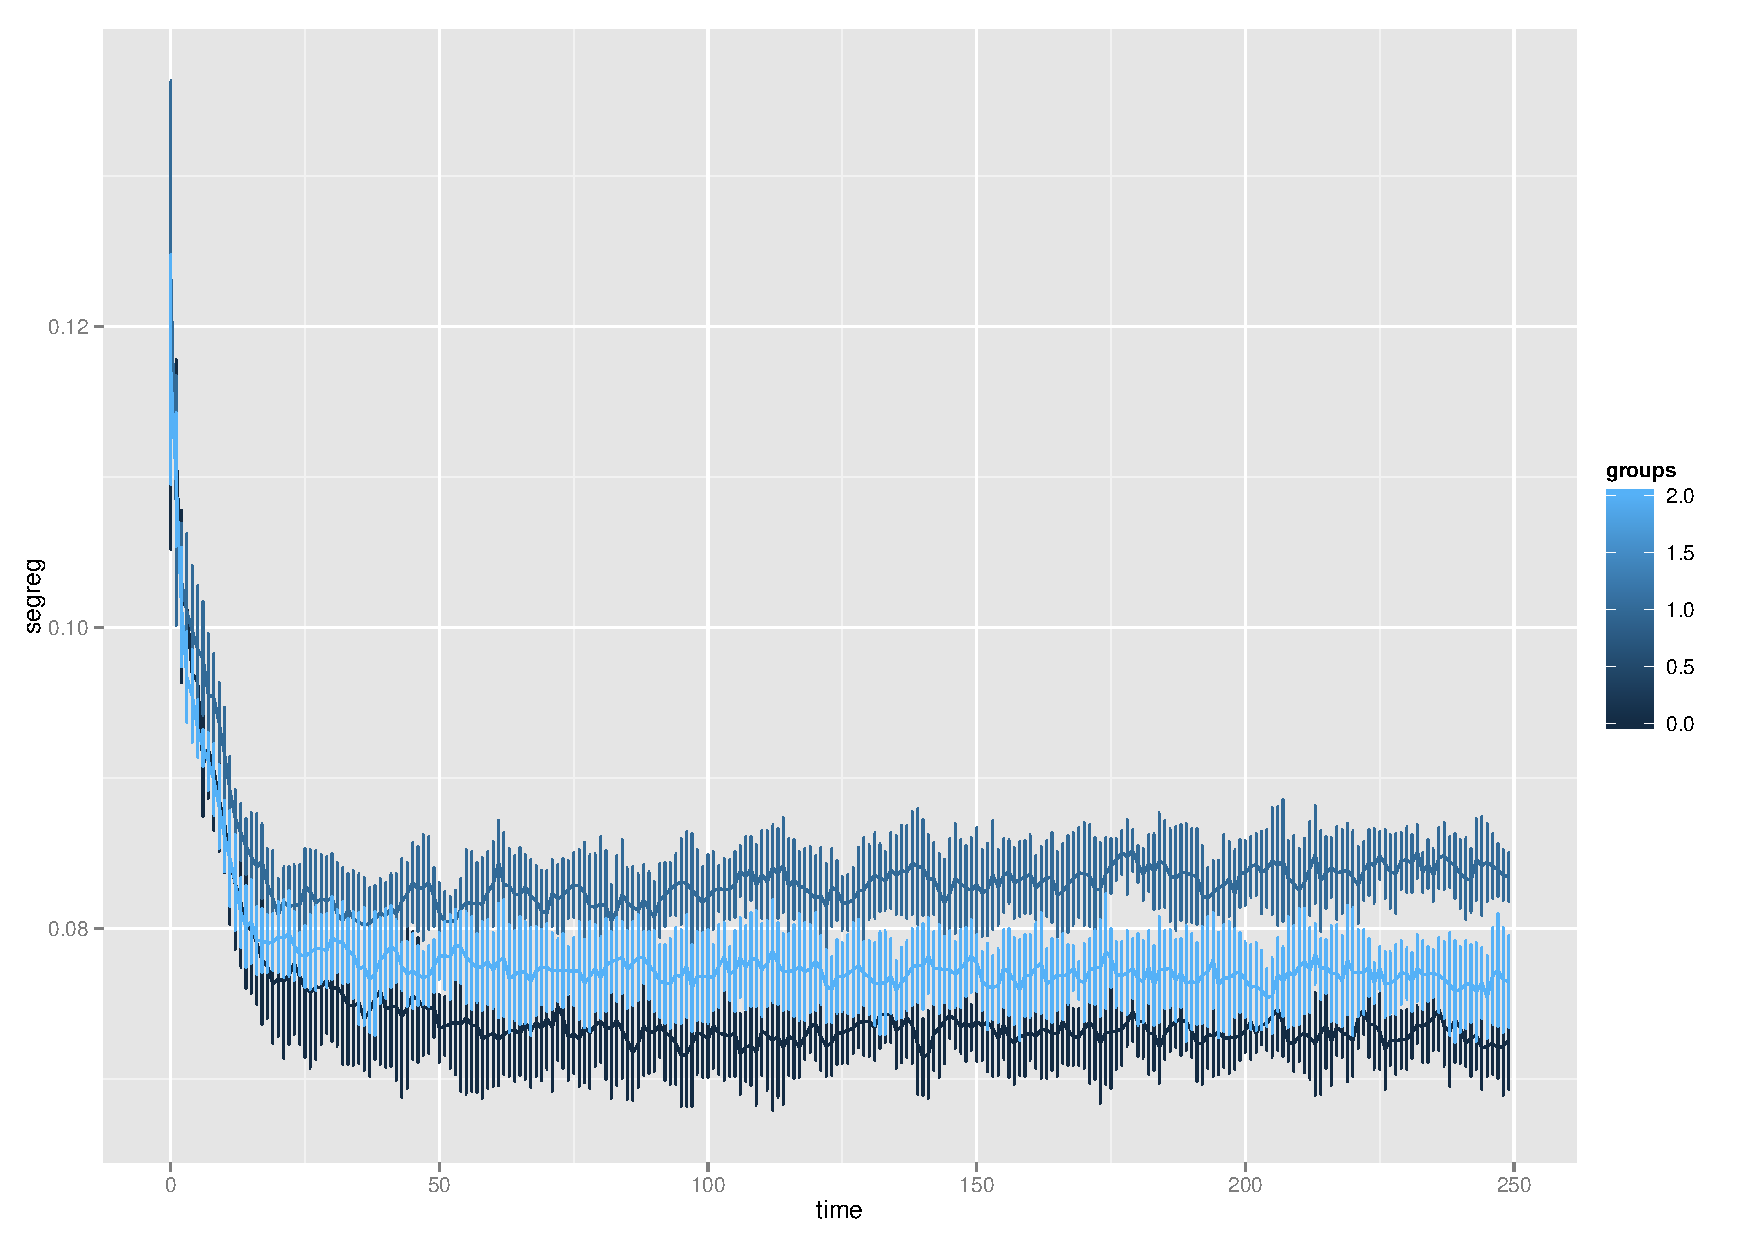
\includegraphics[width=0.8\textwidth]{figures/rbd_ConvergenceSegreg}

\textit{Time series of segregation index during a run of the economic ABM
for different configurations.}
\end{figure}
}




\sframe{Practical application: method}{

\begin{itemize}
\item \begin{justify}Fixing the spatial initial structure and the parameters, optimize
on the possible distribution of activities among centers. Choice of
parameters is crucial.\end{justify}
\vfill{}

\item \begin{justify}Importation of real GIS data: centers correspond to centroids of zones
in a district, initial network to main roads. Some centers have fixed
activity (stations), other can be 2 different ones (residential or
tertiary).\end{justify}
\vfill{}

\item \begin{justify}Exploration of all possible configurations (possible here, $2^{8}=256$
configurations), Pareto-plot of economic performance and accessibility.\end{justify}
\end{itemize}

}



\sframe{Practical application}{

\begin{figure}
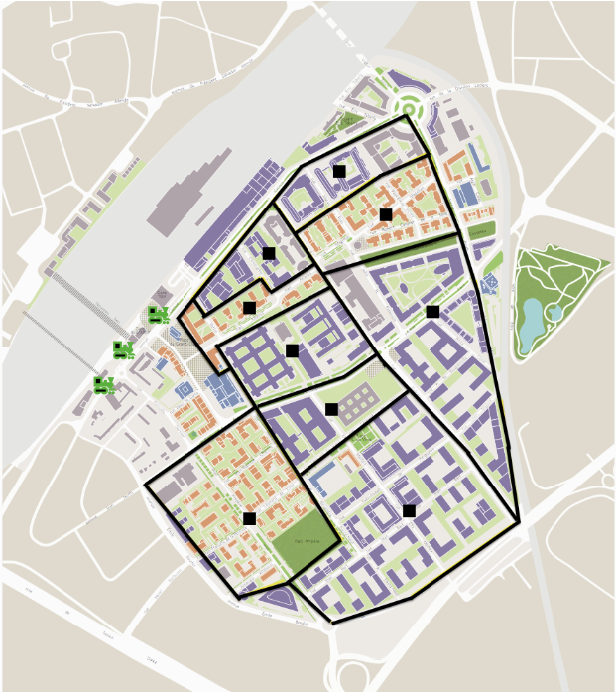
\includegraphics[height=0.5\textwidth]{figures/rbd_RasterAtlantisLast}\hspace{0.5cm}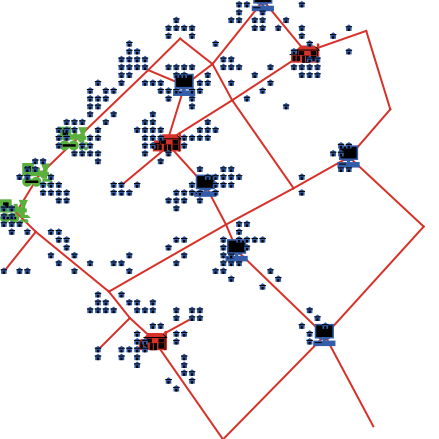
\includegraphics[height=0.5\textwidth]{figures/rbd_ExampleActivitiesRealSituation}
\end{figure}

\textit{Practical application.} Optimizing the distribution of activities over
urban centers.

}


\sframe{Application : Pareto optimization}{
\begin{columns}%{}


\column{7cm}


\begin{figure}[t] \centering 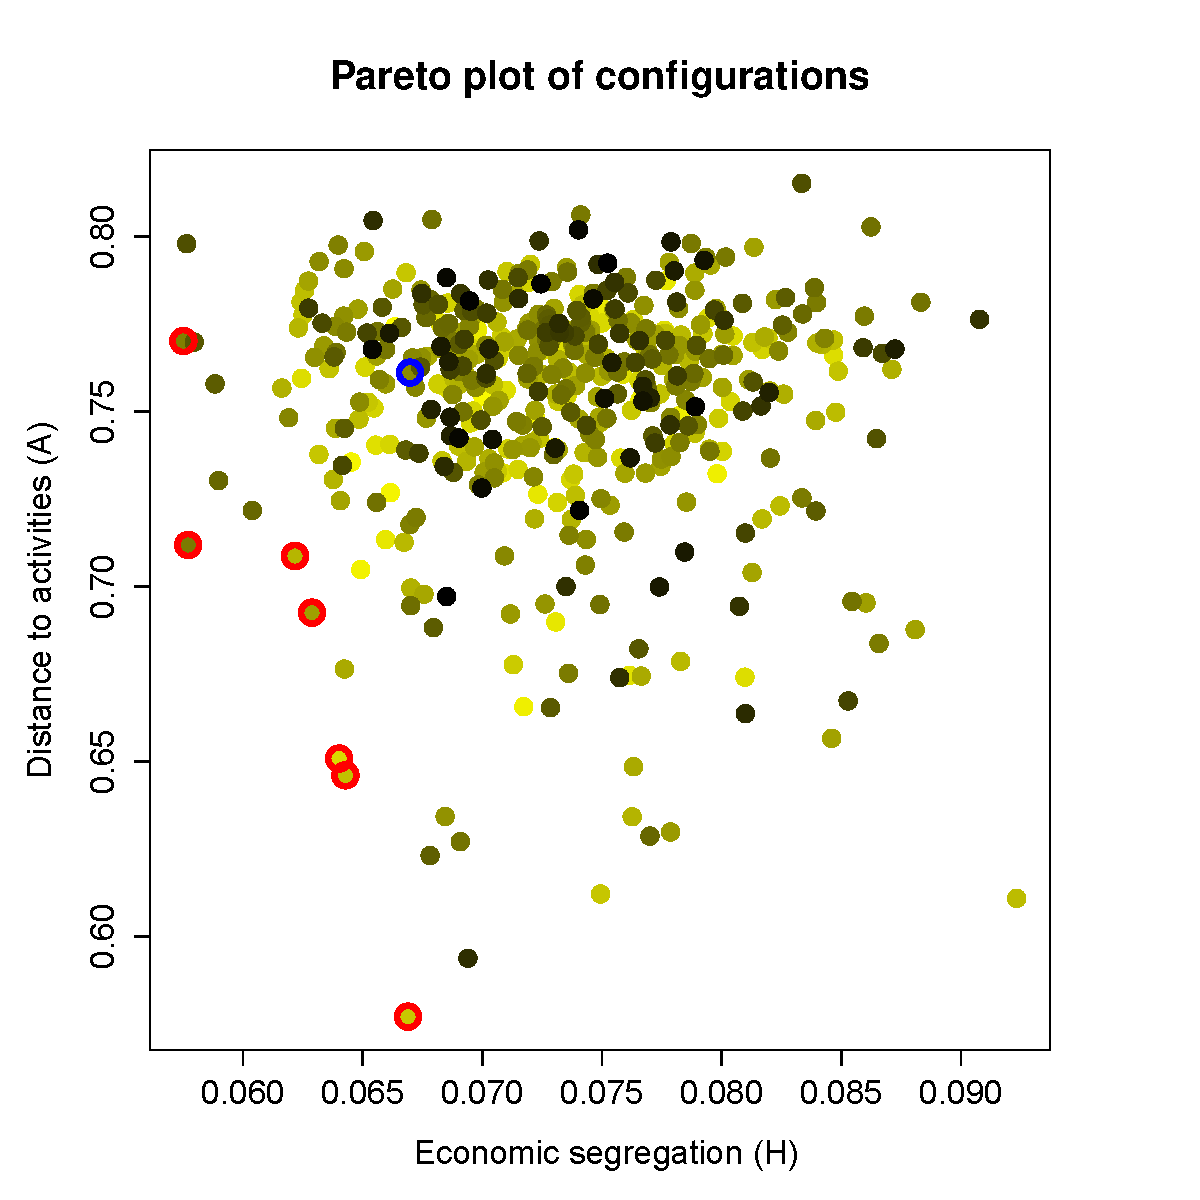
\includegraphics[trim=0mm 0mm 10mm 10mm, clip, width=\columnwidth]{figures/rbd_ParetoLastGoodRealPoint}   \end{figure}


\column{5cm}


\textit{Scatterplot of all configurations in the $(H,A)$ morphological
plane.}


Real situation in blue, Pareto front in red. Color gradient follows
level of heterogeneity from low (black) to high (yellow). It suggests
the performance of functional heterogeneity, often recommended by
planners today.

\end{columns}

}


%\sframe{Discussion}{
%
%\vfill{}
%
%\begin{itemize}
%\item \begin{justify}Many questions are still open: do we have the good scale of application? (although it should be scale-free), did we isolate the dominant
%processes? (cf \cite{2013arXiv1309.3961L})\end{justify}
%\vfill{}
%
%\item \begin{justify}Local scope : is the system isolated? Economic processes are implicitly
%taken into account.\end{justify}
%\vfill{}
%
%\item \begin{justify}Towards a more operational model? Difficulty to calibrate conceptual
%CA models on real data \cite{maria2003stochastic}\end{justify}
%\vfill{}
%
%\item \begin{justify}Complex coupling with economic ABM \cite{varenne2013modeliser}?
%Compromise between complexity level and model performance always difficult
%to find.\end{justify}
%\end{itemize}
%}
%
%\begin{itemize}
%\item \begin{justify}Interesting qualitative and quantitative results: reproduction of
%Le Corbusier's typology; assessment of relative performance of urban
%mixity \cite{mangin2004ville} .\end{justify}
%\vfill{}
%
%\item \begin{justify}Can be seen as going in the sense of the emergence of a rigourous
%``evidence-based urbanism'', or ``quantitative urbanism''\\(\cite{portugali2012complexity}).\end{justify}
%\end{itemize}
% quite naive three years ago...



\sframe{Causality regimes between the network and the city}{

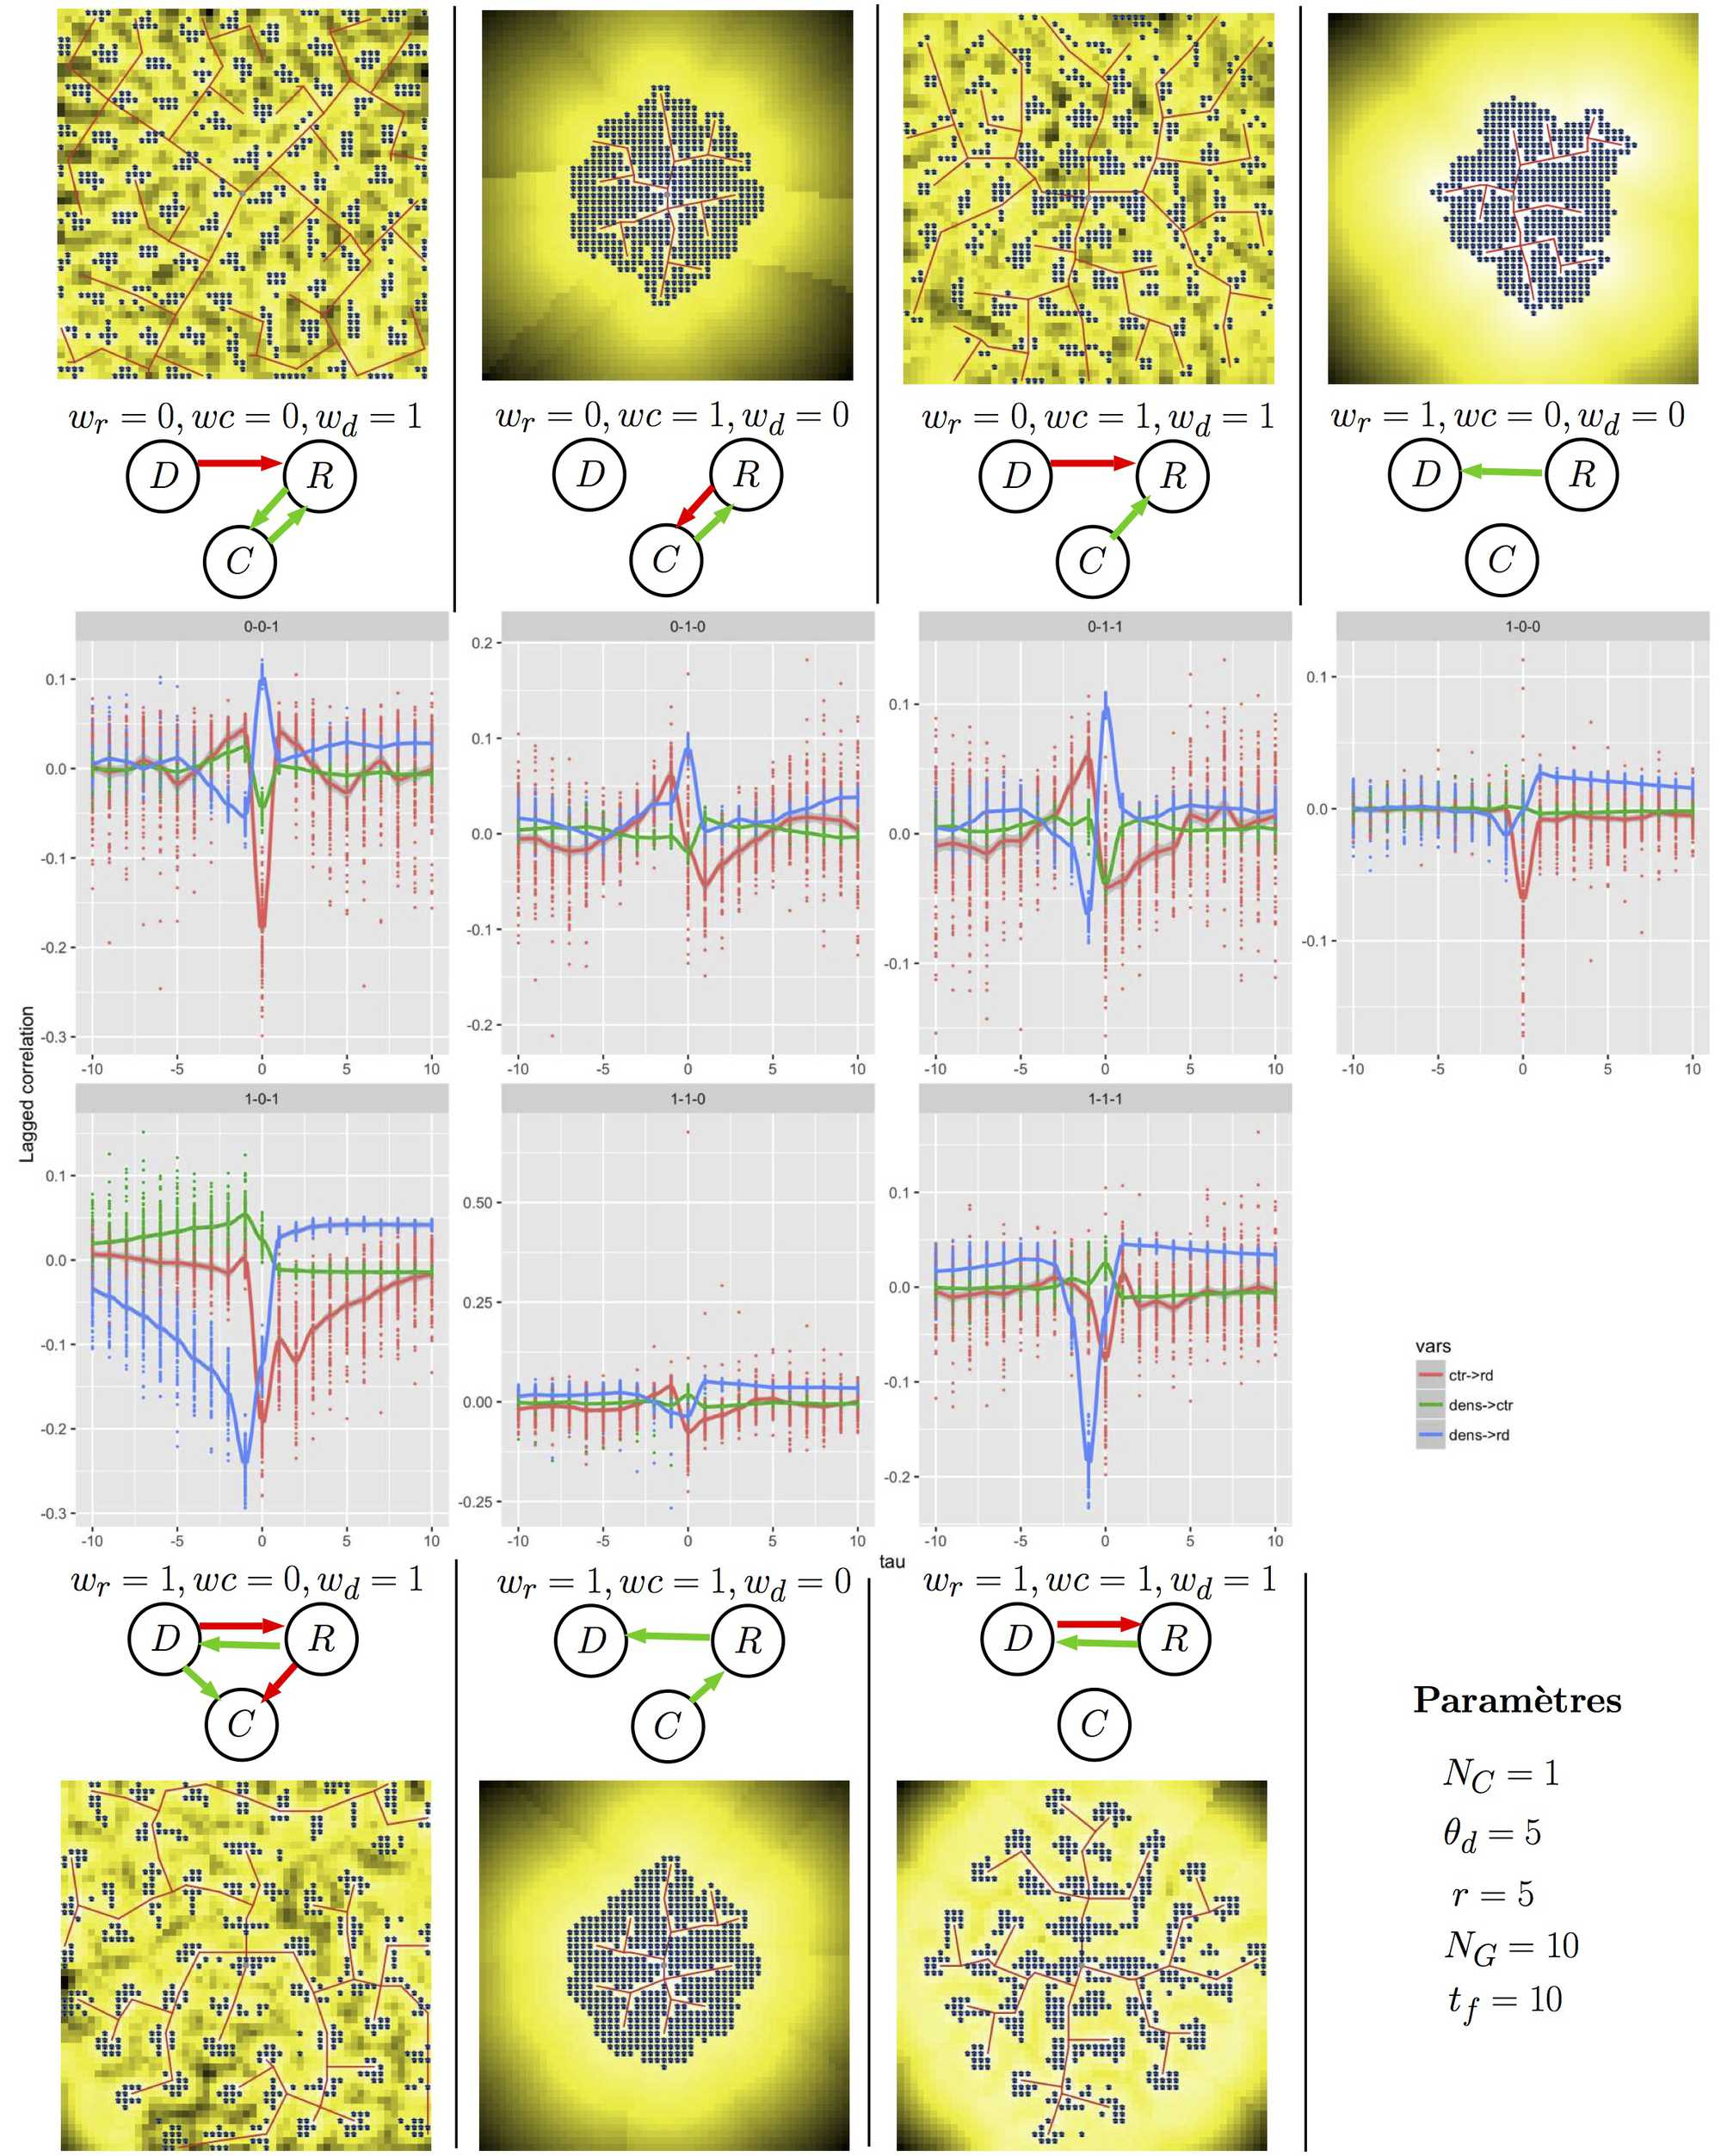
\includegraphics[height=\textheight]{figures/rbd_4-2-2-fig-causalityregimes-exrdb.jpg}

}






\sframe{A Morphogenesis Model of co-evolution}{

\justify

\vspace{-1cm}

$\rightarrow$ Coupled grid population distribution and vector transportation network, following the core of \cite{raimbault2014hybrid}

\medskip

$\rightarrow$ Local morphological and functional variables determine a patch-value, driving new population attribution through preferential attachment ; combined to population diffusion (reaction-diffusion processes studied before)

% Comment Arnaud : réaction-diffusion ?

\medskip

$\rightarrow$ Network growth is also driven by morphological, functional and local network measures, following diverse heuristics corresponding to different processes (multi-modeling)

\bigskip
\bigskip

\textit{Local variables and network properties induce feedback on both, thus a strong coupling capturing the \textbf{co-evolution}}

}



\sframe{Model : Specification}{

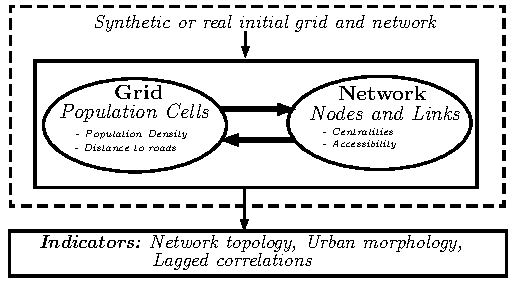
\includegraphics[width=\textwidth]{figures/coevol_mesocoevol}

}



\sframe{Network Generation}{

At fixed time steps :

\begin{enumerate}
	\item Add new nodes preferentially to new population and connect them
	\item \justify Variable heuristic for new links, among: nothing, random, gravity-based deterministic breakdown, gravity-based random breakdown (from \cite{schmitt2014modelisation}), cost-benefits (from \cite{louf2013emergence}), biological network generation (based on \cite{tero2010rules})
\end{enumerate}

\medskip

\centering

\frame{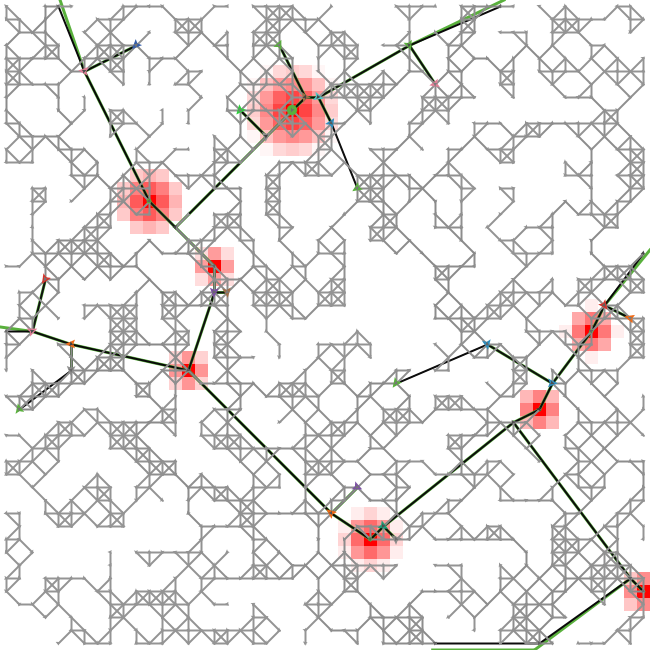
\includegraphics[height=0.31\textwidth]{figures/coevol_example-bio-process-1}}\hspace{0.2cm}
\frame{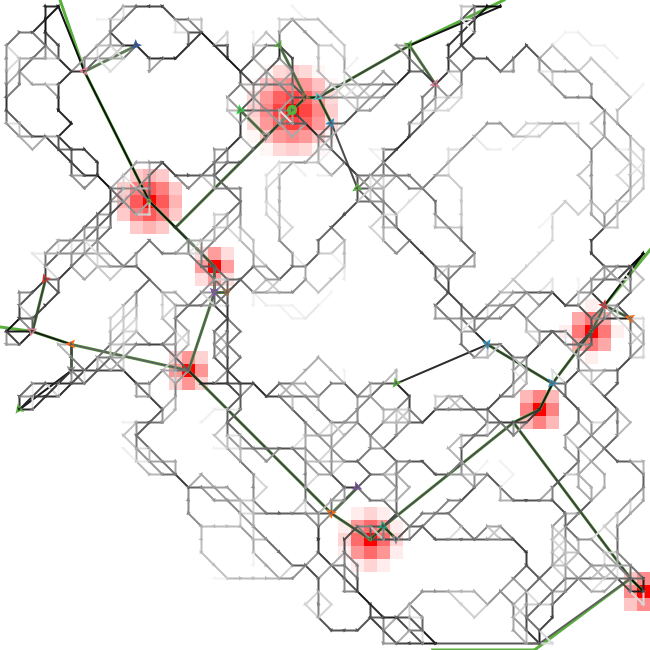
\includegraphics[height=0.31\textwidth]{figures/coevol_example-bio-process-1-tick80}}

\footnotesize

\textit{Intermediate stage for biological network generation}

}




\sframe{Generated Urban Shapes: Urban Form}{

\centering

\frame{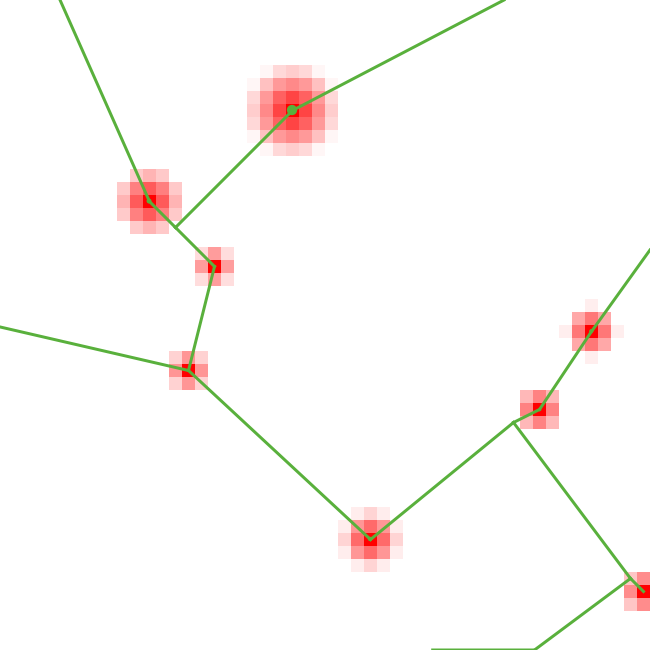
\includegraphics[width=0.28\textwidth]{figures/coevol_example_synthsetup}}\hspace{0.1cm}
\frame{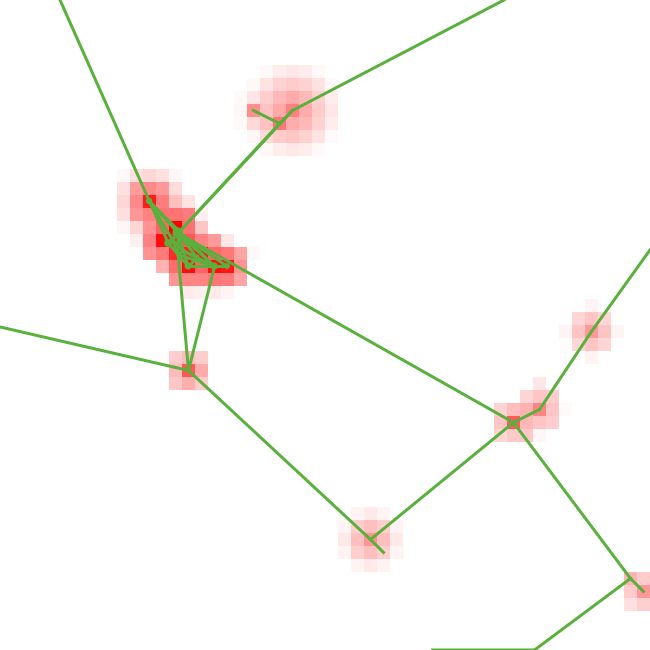
\includegraphics[width=0.28\textwidth]{figures/coevol_example_form-accessonly}}\hspace{0.1cm}
\frame{\includegraphics[width=0.28\textwidth]{figures/coevol_example_form-droadonly}}\\\vspace{0.1cm}
\frame{\includegraphics[width=0.28\textwidth]{figures/coevol_example_form-bwonly}}\hspace{0.1cm}
\frame{\includegraphics[width=0.28\textwidth]{figures/coevol_example_form-closenessonly}}\hspace{0.1cm}
\frame{\includegraphics[width=0.28\textwidth]{figures/coevol_example_form-poponly}}

\footnotesize\textit{In order: setup; accessibility driven; road distance driven; betweenness driven; closeness driven; population driven.}

}






\sframe{Generated Urban Shapes: Network}{


\centering

\frame{\includegraphics[width=0.28\textwidth]{figures/coevol_example_nw-connection}}\hspace{0.1cm}
\frame{\includegraphics[width=0.28\textwidth]{figures/coevol_example_nw-random}}\hspace{0.1cm}
\frame{\includegraphics[width=0.28\textwidth]{figures/coevol_example_nw-gravity}}\\\vspace{0.1cm}
\frame{\includegraphics[width=0.28\textwidth]{figures/coevol_example_nw-rndbrkdwn}}\hspace{0.1cm}
\frame{\includegraphics[width=0.28\textwidth]{figures/coevol_example_nw-cost}}\hspace{0.1cm}
\frame{\includegraphics[width=0.28\textwidth]{figures/coevol_example_nw-bio}}

\footnotesize\textit{In order: connection; random; deterministic breakdown; random breakdown; cost-driven; biological.}

}



\sframe{Results : Network Heuristics}{

\justify

\textit{Comparison of feasible space for network indicators with fixed density}

\bigskip

\includegraphics[width=0.52\textwidth,height=0.6\textheight]{figures/coevol_feasible_space_withreal_pca_bymorph}
\includegraphics[width=0.43\textwidth,height=0.6\textheight]{figures/coevol_distance_real_bymorph}

\footnotesize

\textit{(Left) Feasible spaces by morphological class and network heuristic; (Right) Distribution of distances to topologies of real networks}

}


\sframe{Results : Calibration}{

\justify

\vspace{-0.5cm}

Calibration (model explored with OpenMole~\cite{reuillon2013openmole}, $\sim 10^6$ model runs) at the first order on morphological and topological objectives, and on correlations matrices.

\bigskip

\begin{columns}
\column{0.4\textwidth}
\centering
\includegraphics[width=\textwidth]{figures/coevol_pca_allobjs}
\column{0.2\textwidth}
\includegraphics[width=\textwidth]{figures/coevol_pca_morpho_byheuristic}\\
\includegraphics[width=\textwidth]{figures/coevol_pca_network_byheuristic}
\column{0.4\textwidth}
\includegraphics[width=\textwidth]{figures/coevol_corrs-distrib_rhoasize4}

\end{columns}

\footnotesize\textit{(Left) Full indicator space; (Middle) Morphological and Topology, by network heuristic; (Right) Distance distribution for cumulated distance for indicators and correlations.}

}


\sframe{Results : Causality Regimes}{

\textit{Unsupervised learning on lagged correlations between local variables unveils a diversity of causality regimes}

$\rightarrow$ Link between \emph{co-evolution regime} and morphogenetic properties of the urban system

% comment Arnaud : le genre d’affirmation qu’il faut réussir à exprimer également du point de vue de l’objet étudié : qu’est-ce que ça veut dire pour la morphogénèse urbaine ?

\medskip

\centering

\includegraphics[width=0.52\textwidth,height=0.55\textheight]{figures/coevol_centertrajs}
\includegraphics[width=0.4\textwidth,height=0.55\textheight]{figures/coevol_cluster-params}

\footnotesize\textit{(Left) Lagged correlation profiles of cluster centers; (Right) Distribution of regimes across parameter space}

}






\sframe{What is Morphogenesis ? Examples}{

% illustrations : ants, geomorphology, neurons, self-assembly ; ARBOTRON ; paper nature aile avion
% all from netlogo library ? would be nice illustration of generative nature


% remark : do not put classical biological example to show how it has percolated to other fields

\vspace{-0.3cm}

\includegraphics[width=\textwidth,height=0.82\textheight]{figures/intro_examples}

\justify

\vspace{-0.5cm}

\footnotesize\textit{Sources (in order by column). Ants, Erosion, Game of Life: NetLogo Library ; Arbotron \cite{jun2005formation}; Industrial design \cite{Aage:2017aa}; Swarm chemistry \cite{sayama2007decentralized}}
% sources : ants netlogo ; erosion netlogo ; arbotron 
%  inge : 

}





\sframe{Defining Morphogenesis}{

% precise notions and defs

\justify

\textit{Construction of an interdisciplinary definition in~\cite{antelope2016interdisciplinary}}

\bigskip




\textbf{Meta-epistemological framework of imbricated notions:}

Self-organization $\supsetneq$ Morphogenesis $\supsetneq$ Autopoiesis $\supsetneq$ Life


\bigskip

\textbf{Properties:}

\begin{itemize}
\item Architecture links form and function
\item Emergence strength~\cite{bedau2002downward} increases with notion depth, as bifurcations~\cite{thom1974stabilite}
\end{itemize}

\bigskip

\textbf{Definition of Morphogenesis :} \textit{Emergence of the form and the function in a strongly coupled manner, producing an emergent architecture \cite{doursat2012morphogenetic}}



}







\sframe{Discussion}{

\justify

\vspace{-1cm}

\textbf{Implications}

$\rightarrow$ This rather simple model reproduces most of existing urban forms in Europe for both population distribution and road network : which intrinsic dimension to the urban system and its morphological aspect ?

$\rightarrow$ Ability to reproduce static correlations and a variety of dynamical lagged correlation regimes suggests that the model captures some of the processes of co-evolution

% implications for morphogenesis ?

\bigskip

\textbf{Developments}


$\rightarrow$ Towards a dynamical calibration ? Need of dynamical data

$\rightarrow$ Investigate the link between spatial non-stationarity and non-ergodicity through simulation by the model

$\rightarrow$ Compare network generation in a ``fair'' way (correcting for additional parameters, open question for models of simulation)


}



\sframe{Conclusion}{


\justify

$\rightarrow$ A novel model of urban morphogenesis at the mesoscopic scale systematically explored : \textbf{need for more coupling and comparison of models.}

\medskip

$\rightarrow$ At the macro scale of the system of cities ? \textbf{Need for multi-scale models.}

\medskip

$\rightarrow$ With more refined urban characteristics and other dimensions ? \textbf{Need for more interdisciplinarity.}

\bigskip
\bigskip
\bigskip

\footnotesize{ - Code, data and results available at\\ \texttt{https://github.com/JusteRaimbault/CityNetwork}\\
- Paper on arXiv at \texttt{https://arxiv.org/abs/1708.06743}\\
- Acknowledgments : We thank the \textit{European Grid Infrastructure} and its \textit{National Grid Initiatives} (\textit{France-Grilles} in particular) to give the technical support and the infrastructure.

}

}






\sframe{Reserve slides}{

\centering

\Large

\textbf{Reserve Slides}

}




%%%%%%%%%%%%%%%%%
%\section*{Morphogenesis}



\sframe{Morphogenesis Overview}{
% other numerous examples of fields/case of application

\cite{bourgine2010morphogenesis} : interdisciplinary workshop on morphogenesis

\bigskip

$\rightarrow$\textit{To what extent the notion is indeed transdisciplinary, i.e. are there common definitions across disciplines ? What are the concepts shared or the divergence ?}


\begin{itemize}
\item \textbf{Biology}
\begin{itemize}
\item External phenotype morphogenesis (ant colony)~\cite{minter2012morphogenesis} \item Symbiosis of species~\cite{chapman1998morphogenesis}
\item Botany~\cite{lord1981cleistogamy}
\end{itemize}
\item \textbf{Social Sciences} : Archeology~\cite{renfrew1978trajectory}
\item \textbf{Epistemology} : \cite{gilbert2003morphogenesis}
\item \textbf{Artificial Intelligence} : From self-assembly to Morphogenetic Engineering~\cite{doursat2013review}. Synthetic Biology ?
\item \textbf{Geomorphology} : dunes formation~\cite{douady2011dunes}
\item \textbf{Physics} : Arbotrons playing Tetris ?
\item etc\ldots
\end{itemize}




}



\sframe{Morphogenesis concepts}{

\begin{itemize}
\item \justify \textbf{Morphogenesis and Self-Organisation} : when does a system exhibit an architecture ? Insights from Morphogenetic Engineering
\cite{doursat2013review}. Architecture : the relation between the form and the function ?
\medskip
\end{itemize}
\begin{itemize}
\item \justify\textbf{Scales, Units and Boundaries} From local interactions to global information flow (Holland's \emph{signal and boundaries}~\cite{holland2012signals}: morphogenesis as the development of Complex Adaptive Systems ?)
\medskip
\end{itemize}
\begin{itemize}
\item \justify \textbf{Symmetry and Bifurcations} : on quantitative becoming qualitative. Ren{\'e} Thom's \emph{theory of catastrophes}~\cite{thom1974stabilite}
\medskip
\end{itemize}
\begin{itemize}
\item \justify \textbf{Life and Death} : link with autopoiesis and cognition\\
\cite{bourgine2004autopoiesis} ; co-evolution of subsystems as an alternative definition ? In psychology, attractors of the mind.
\end{itemize}


}


\sframe{Catastrophe Theory}{

% brief rapide sur theorie des catastrophes

A system is viewed as its internal state $X_w$, where $w\in W$ is a control parameter.

\bigskip

Catastrophe set $K \subset W$ is where the system endures phase transition.

\bigskip

Thom classified possible topologies for $K$ depending on the dimension of $W$.

}






%%%%%%%%%%%%%%%%%
%\section*{Density Morphogenesis}





\sframe{Model classification : PDE}{

% derived PDE

The one-dimensional model verifies the PDE :

\begin{equation}\label{eq:pde}
\begin{split}
\delta t \cdot \frac{\partial p}{\partial t} = \frac{N_G \cdot p^{\alpha}}{P_{\alpha}(t)} + \frac{\alpha \beta (\alpha - 1) \delta x^2}{2}\cdot \frac{N_G \cdot p^{\alpha-2}}{P_{\alpha}(t)} \cdot \left(\frac{\partial p}{\partial x}\right)^2\\
+ \frac{\beta \delta x^2}{2} \cdot \frac{\partial^2 p}{\partial x^2} \cdot\left[ 1 + \alpha \frac{N_G p^{\alpha - 1}}{P_{\alpha(t)}} \right]
\end{split}
\end{equation}

}


\sframe{Stationary behavior of 1D model}{
\centering
\includegraphics[width=\textwidth]{figures/density_stationary}
}

\sframe{Stationary behavior of 1D model}{
\centering
\includegraphics[width=0.48\textwidth]{figures/density_pmax_alpha}
\includegraphics[width=0.48\textwidth]{figures/density_pmax_logbeta}

}



\sframe{Morphological indicators}{

\begin{enumerate}
\item Rank-size slope $\gamma$, given by $\ln \left( P_{\tilde{i}}/P_0\right) \sim k + \gamma\cdot \ln \left(\tilde{i}/i_0\right)$ where $\tilde{i}$ are the indexes of the distribution sorted in decreasing order.
\item Entropy of the distribution:
\begin{equation}
\mathcal{E} = \sum_{i=1}^{M}\frac{P_i}{P}\cdot \ln{\frac{P_i}{P}}
\end{equation}
$\mathcal{E}=0$ means that all the population is in one cell whereas $\mathcal{E}=0$ means that the population is uniformly distributed.
\item Spatial-autocorrelation given by Moran index, with simple spatial weights given by $w_{ij} = 1/d_{ij}$
\[
I = M \cdot \frac{\sum_{i\neq j} w_{ij} \left(P_i - \bar{P}\right)\cdot\left(P_j - \bar{P}\right)}{\sum_{i\neq j} w_{ij} \sum_{i}{\left( P_i - \bar{P}\right)}^2}
\]
\item Mean distance between individuals
\[
\bar{d} = \frac{1}{d_M}\cdot \sum_{i<j} \frac{P_i P_j}{P^2} \cdot d_{ij}
\]
where $d_M$ is a normalisation constant
\end{enumerate}



}


\sframe{Model behavior : Convergence}{

Large number of repetitions show good convergence properties

% hist examples

\includegraphics[width=0.5\textwidth]{figures/density_hist_moran}
\includegraphics[width=0.5\textwidth]{figures/density_hist_slope}

}


\sframe{Model behavior}{


\includegraphics[width=0.5\textwidth]{figures/density_pc_colalpha}
\includegraphics[width=0.5\textwidth]{figures/density_pc_colbeta}

}


\sframe{Empirical indicators computation}{

$\rightarrow$ Eurostat population density raster (100m, simplified at 500m resolution)

\medskip

$\rightarrow$ Overlapping (10km offset) squares of 50km side : equivalent to smoothing, removes window shape effect. Not very sensitive to window size (tested with 30km and 100km)

\medskip

$\rightarrow$ Indicators computed using Fast Fourier Transform Convolution

\medskip

$\rightarrow$ Classification using repeated k-means ; number of clusters taken at transition in clustering coefficient.

}

\sframe{Model calibration: all indicators}{

\centering
\includegraphics[width=0.8\textwidth]{figures/density_scatter}

}




%%%%%%%%%%%%%%%%%
%\section*{Co-evolution Morphogenesis}




\sframe{Defining co-evolution}{


\justify

No clear definition of co-evolution in the literature : \cite{bretagnolle:tel-00459720} distinguishes ``reciprocal adaptation'' where a sense of causality can clearly be identified, from co-evolutive regimes 


\bigskip
\bigskip

Identification of multiple causality regimes in a simple strongly coupled growth model $\rightarrow$ to be put in perspective with a theoretical definition of co-evolution based on the conjunction of Morphogenesis and the Evolutive Urban Theory, summarised by~\cite{raimbault2017co}

}


\sframe{Modeling Co-evolution}{

\justify

\cite{baptistemodeling} system dynamics with evolving capacities
 
\cite{wu2017city} population diffusion and network growth

\cite{blumenfeld2010network} and \cite{schmitt2014modelisation} : random potential breakdown for network growth.

\cite{barthelemy2009co} geometrical network growth model making network topology co-evolve with vertex density

}


\sframe{Empirical Data : network indicators}{

\centering

\includegraphics[width=0.53\textwidth]{figures/coevol_FR_indics_network_selected_2_discrquantiles}

}

\sframe{Empirical Data : correlations}{

\centering
\includegraphics[width=0.7\textwidth]{figures/coevol_FR_corr_PCA_rhoasize12}

}



\sframe{Network Indicators}{

Network Topology measured by:

\begin{itemize}
	\item Betweenness and Closeness centralities: average and hierarchy
	\item Accessibility (weighted closeness)
	\item Efficiency (network pace relative to euclidian distance)
	\item Mean path length, diameter
\end{itemize}

}




\sframe{Model specification}{

\footnotesize

Patch utility given by $U_i = \sum_k w_k \cdot \tilde{x}_k$ with $\tilde{x}_k$ normalized local variables among population, betweenness and closeness centrality, distance to roads, accessibility ; aggregation done with probability $\left(U_i/\sum_k U_k\right)^\alpha$ ; diffusion among neighbors $n_d$ times with strength $\beta$

\medskip

\textbf{Network Generation :}

Adding a fixed number $n_N$ of new nodes : for patches such that $d_r < d_0$, probability to receive a node is

%% note : not a proba for the last ? no pb as soon as in 0,1, realized anyway.
\[
p = P/P_{max} \cdot (d_M - d)/d_M \cdot \exp\left(-((d_r - d_0)/\sigma_r)^2\right)
\]

Nodes connected the shortest way to existing network.

\medskip

\textbf{General model parameters :}

\begin{itemize}
	\item Patch utility weights $w_k$
	\item General network generation parameters: growth time steps $t_N$, maximal additional links
\end{itemize}

}



\sframe{Deterministic breakdown Network generation}{

\begin{enumerate}
\item Gravity potential given by
\[
V_{ij}(d) = \left[ (1 - k_h) + k_h \cdot \left( \frac{P_i P_j}{P^2} \right)^{\gamma} \right]\cdot \exp{\left( -\frac{d}{r_g (1 + d/d_0)} \right)}
\]

\item $k\cdot N_L$ links are selected with lowest $V_{ij}(d_N)/V_{ij}(d_{ij})$, among which $N_L$ links with highest (lest costly) are realized
\item Network is planarized
\end{enumerate}
}


\sframe{Biological Network generation}{

Adding new links with biological heuristic:

\begin{enumerate}
	\item Create network of potential new links, with existing network and randomly sampled diagonal lattice
	\item Iterate for $k$ increasing ($k\in \{ 1,2,4 \}$ in practice) :
	\begin{itemize}
		\item Using population distribution, iterate $k\cdot n_b$ times the slime mould model to compute new link capacities
		\item Delete links with capacity under $\theta_d$
		\item Keep the largest connected component
	\end{itemize}
	\item Planarize and simplify final network
\end{enumerate}

}


\sframe{Model setup}{

\textbf{Synthetic setup: } rank-sized monocentric cities, simple connection with bord nodes to avoid bord effects 

\textbf{Real setup: } Population density raster at 500m resolution (European Union, from Eurostat)

\centering
\frame{\includegraphics[width=0.35\textwidth]{figures/coevol_example_synthsetup}}\hspace{0.1cm}
\frame{\includegraphics[width=0.35\textwidth]{figures/coevol_example-realsetup}}

\textbf{Stopping conditions: } fixed final time; fixed total population; fixed network size.

}


\sframe{Calibration Method}{


%% The model is calibrated at the first order (indicators of urban form and network measures) and at the second order (correlations) with Eurostat population grid coupled with street network from OpenStreetMap through the following workflow: indicators (Moran index, mean distance, hierarchy, entropy for morphology, mean path length, centralities, performance for network) are computed on real areas of width 50km for all Europe (what corresponds to the typical scale of processes the model includes); parameter space of the model is explored using grid computing (with OpenMole model exploration software), from simple synthetic initial configurations (few connected punctual settlements), computing indicators on final simulated configurations;  among candidate parameters for given contiguous (in space and indicator space) real areas on which correlations can be computed, the one with the closest correlation matrix computed on repetitions is chosen.



\begin{itemize}
	\item Brute force exploration of a LHS sampling, 10 repetitions of the model for each parameter point.
	\item For each simulated point, closest in indicator space (euclidian distance for normalized indicators) among real points are selected.
	\item Among these, point with lowest distance to correlation matrix are taken.
\end{itemize}


}

\sframe{Calibration : optimal points}{

\centering

\includegraphics[width=0.45\textwidth]{figures/coevol_dists_pareto_i1}
\includegraphics[width=0.45\textwidth]{figures/coevol_dists_pareto_i10}

\footnotesize\textit{Pareto plots of distance to indicators and distance to correlation matrices, for a given simulated configuration and all real points.}

}



\sframe{Causality regimes: clustering}{

\centering

\includegraphics[width=0.48\textwidth]{figures/coevol_clustcoef}
\includegraphics[width=0.48\textwidth]{figures/coevol_diffclustcoef}

\medskip

\footnotesize\textit{Clustering coefficient (left) and its derivative (right) as a function of number of clusters}

}





\sframe{Co-evolution Models}{

\centering
\includegraphics[width=0.8\textwidth]{figures/thematic_coevolution}

}





%%%%%%%%%%%%%%%%%%%%%
\begin{frame}[allowframebreaks]
\frametitle{References}
\bibliographystyle{apalike}
\bibliography{/Users/juste/ComplexSystems/CityNetwork/Biblio/Bibtex/CityNetwork,biblio,biblio_morphogen,ccupd,global,projetCSMS,dynamite}
\end{frame}
%%%%%%%%%%%%%%%%%%%%%%%%%%%%




\end{document}







